% ============================================================================
% ch3-results.tex — Chapter III: Results
% V4: sequential exhibits, enriched Discussion, Amundi reference
% ============================================================================
\chapterpage{Chapter\kern0.25em III}{Results}{images/IM3.jpeg}
\thispagestyle{chapterstart}

\noindent\textit{US\$388 billion. That is the climate risk embedded in today's installed data center base---38\% of enterprise value, invisible in standard valuations. This chapter presents four findings at macroeconomic scale, three facility case studies, and an interpretation of results. All figures use the BAU climate-economic pathway and MEAN estimates unless noted otherwise.}

\vspace{4mm}

% ---- Panoramic table ----
\exhibitcaption{10}{Panoramic results: ClimVaR across asset classes, AI scenarios, and adaptation strategies (BAU/MEAN).}

\begin{center}
\datatablesetup
\begin{tabularx}{\textwidth}{>{\raggedright\arraybackslash}p{3.5cm} >{\raggedleft\arraybackslash}X >{\raggedleft\arraybackslash}X >{\raggedleft\arraybackslash}X >{\raggedleft\arraybackslash}X >{\raggedleft\arraybackslash}X}
\toprule
\datatableheader
\thd{Portfolio} & \thd{V$_0$ (\$B)} & \thd{Baseline} & \thd{Selective} & \thd{Proactive} & \thd{Max red.} \\
\midrule
\textbf{Installed base} & \textbf{1,012} & \textbf{388} (38\%) & \textbf{305} (30\%) & \textbf{238} (24\%) & \textbf{39\%} \\
\quad United States & 393 & 108 (28\%) & 89 (23\%) & 72 (18\%) & 33\% \\
\quad Europe & 201 & 107 (53\%) & 81 (40\%) & 60 (30\%) & 44\% \\
\quad China & 198 & 111 (56\%) & 86 (44\%) & 67 (34\%) & 40\% \\
\quad APMEA & 220 & 62 (28\%) & 49 (22\%) & 39 (18\%) & 37\% \\
\midrule
\textbf{Installed + LTG} & \textbf{1,992} & \textbf{1,008} (51\%) & \textbf{821} (41\%) & \textbf{669} (34\%) & \textbf{34\%} \\
\textbf{Installed + SAI} & \textbf{2,849} & \textbf{1,669} (59\%) & \textbf{1,366} (48\%) & \textbf{1,134} (40\%) & \textbf{32\%} \\
\textbf{Installed + AWB} & \textbf{5,590} & \textbf{3,671} (66\%) & \textbf{3,006} (54\%) & \textbf{2,536} (45\%) & \textbf{31\%} \\
\bottomrule
\end{tabularx}
\datatableclear
\end{center}

\exhibitsource{ClimVaR\% in parentheses = ClimVaR as \% of V$_0$. Max reduction = (Baseline $-$ Proactive) / Baseline. Under NZT, installed base ClimVaR rises to \$845B (83\%), with Proactive reducing it by 52\%.}

\begin{twocolbody}

\noindent Three patterns structure the results that follow.

\textbf{First, the absolute exposure is large.} The installed base of 8,572 data centers carries \$388~billion in climate-related value at risk---38.3\% of enterprise value under the BAU pathway. This figure rises to \$1.0--3.7~trillion when prospective AI infrastructure is included, depending on growth scenario. Even the most conservative scenario (Limits to Growth) produces over \$1~trillion in exposure. To put this in perspective: \$388B exceeds the annual revenue of every listed data center operator combined.

\textbf{Second, risk is not uniform.} Europe and China face 53--56\% ClimVaR intensity while the United States faces 28\%---a twofold dispersion that reflects not just geographic hazard variation but fundamentally different channel compositions. BI dominates in the US; carbon in Europe; physical damage in Asia-Pacific. Treating ``data center climate risk'' as a single category obscures the specific levers available in each market.

\textbf{Third, ClimVaR intensity rises with AI scale.} Installed base intensity is 38\%; with AI infrastructure, it climbs to 51\% (LTG), 59\% (SAI), or 66\% (AWB). This is not a proportional increase---it reflects the structural inversion from carbon-dominated to physically-dominated risk documented in Finding~4. Each additional GW of AI capacity carries more climate risk per unit than the last.

A note on interpretation: ClimVaR figures represent cumulative discounted value erosion over asset lifetimes, not instantaneous shocks. A ClimVaR of 38\% means that, accounting for cooling penalties, carbon costs, business interruption, physical damage, and heat productivity losses over 25 years, the risk-adjusted present value is 38\% lower than the climate-naive valuation. This is directly comparable to a credit impairment or a perpetual margin compression---it is not a probability of catastrophic loss, but a structural repricing of the asset.

\end{twocolbody}

% ---- Sankey page ----
\clearpage\thispagestyle{chapterstart}

\subsection*{The Transmission Mechanism}
\sectionsubtitle{How seven climate hazards propagate through four risk channels to erode US\$388 billion}
\greensep

\exhibitcaption{11}{From hazard to enterprise value loss: the ClimVaR transmission map.}
\begin{center}
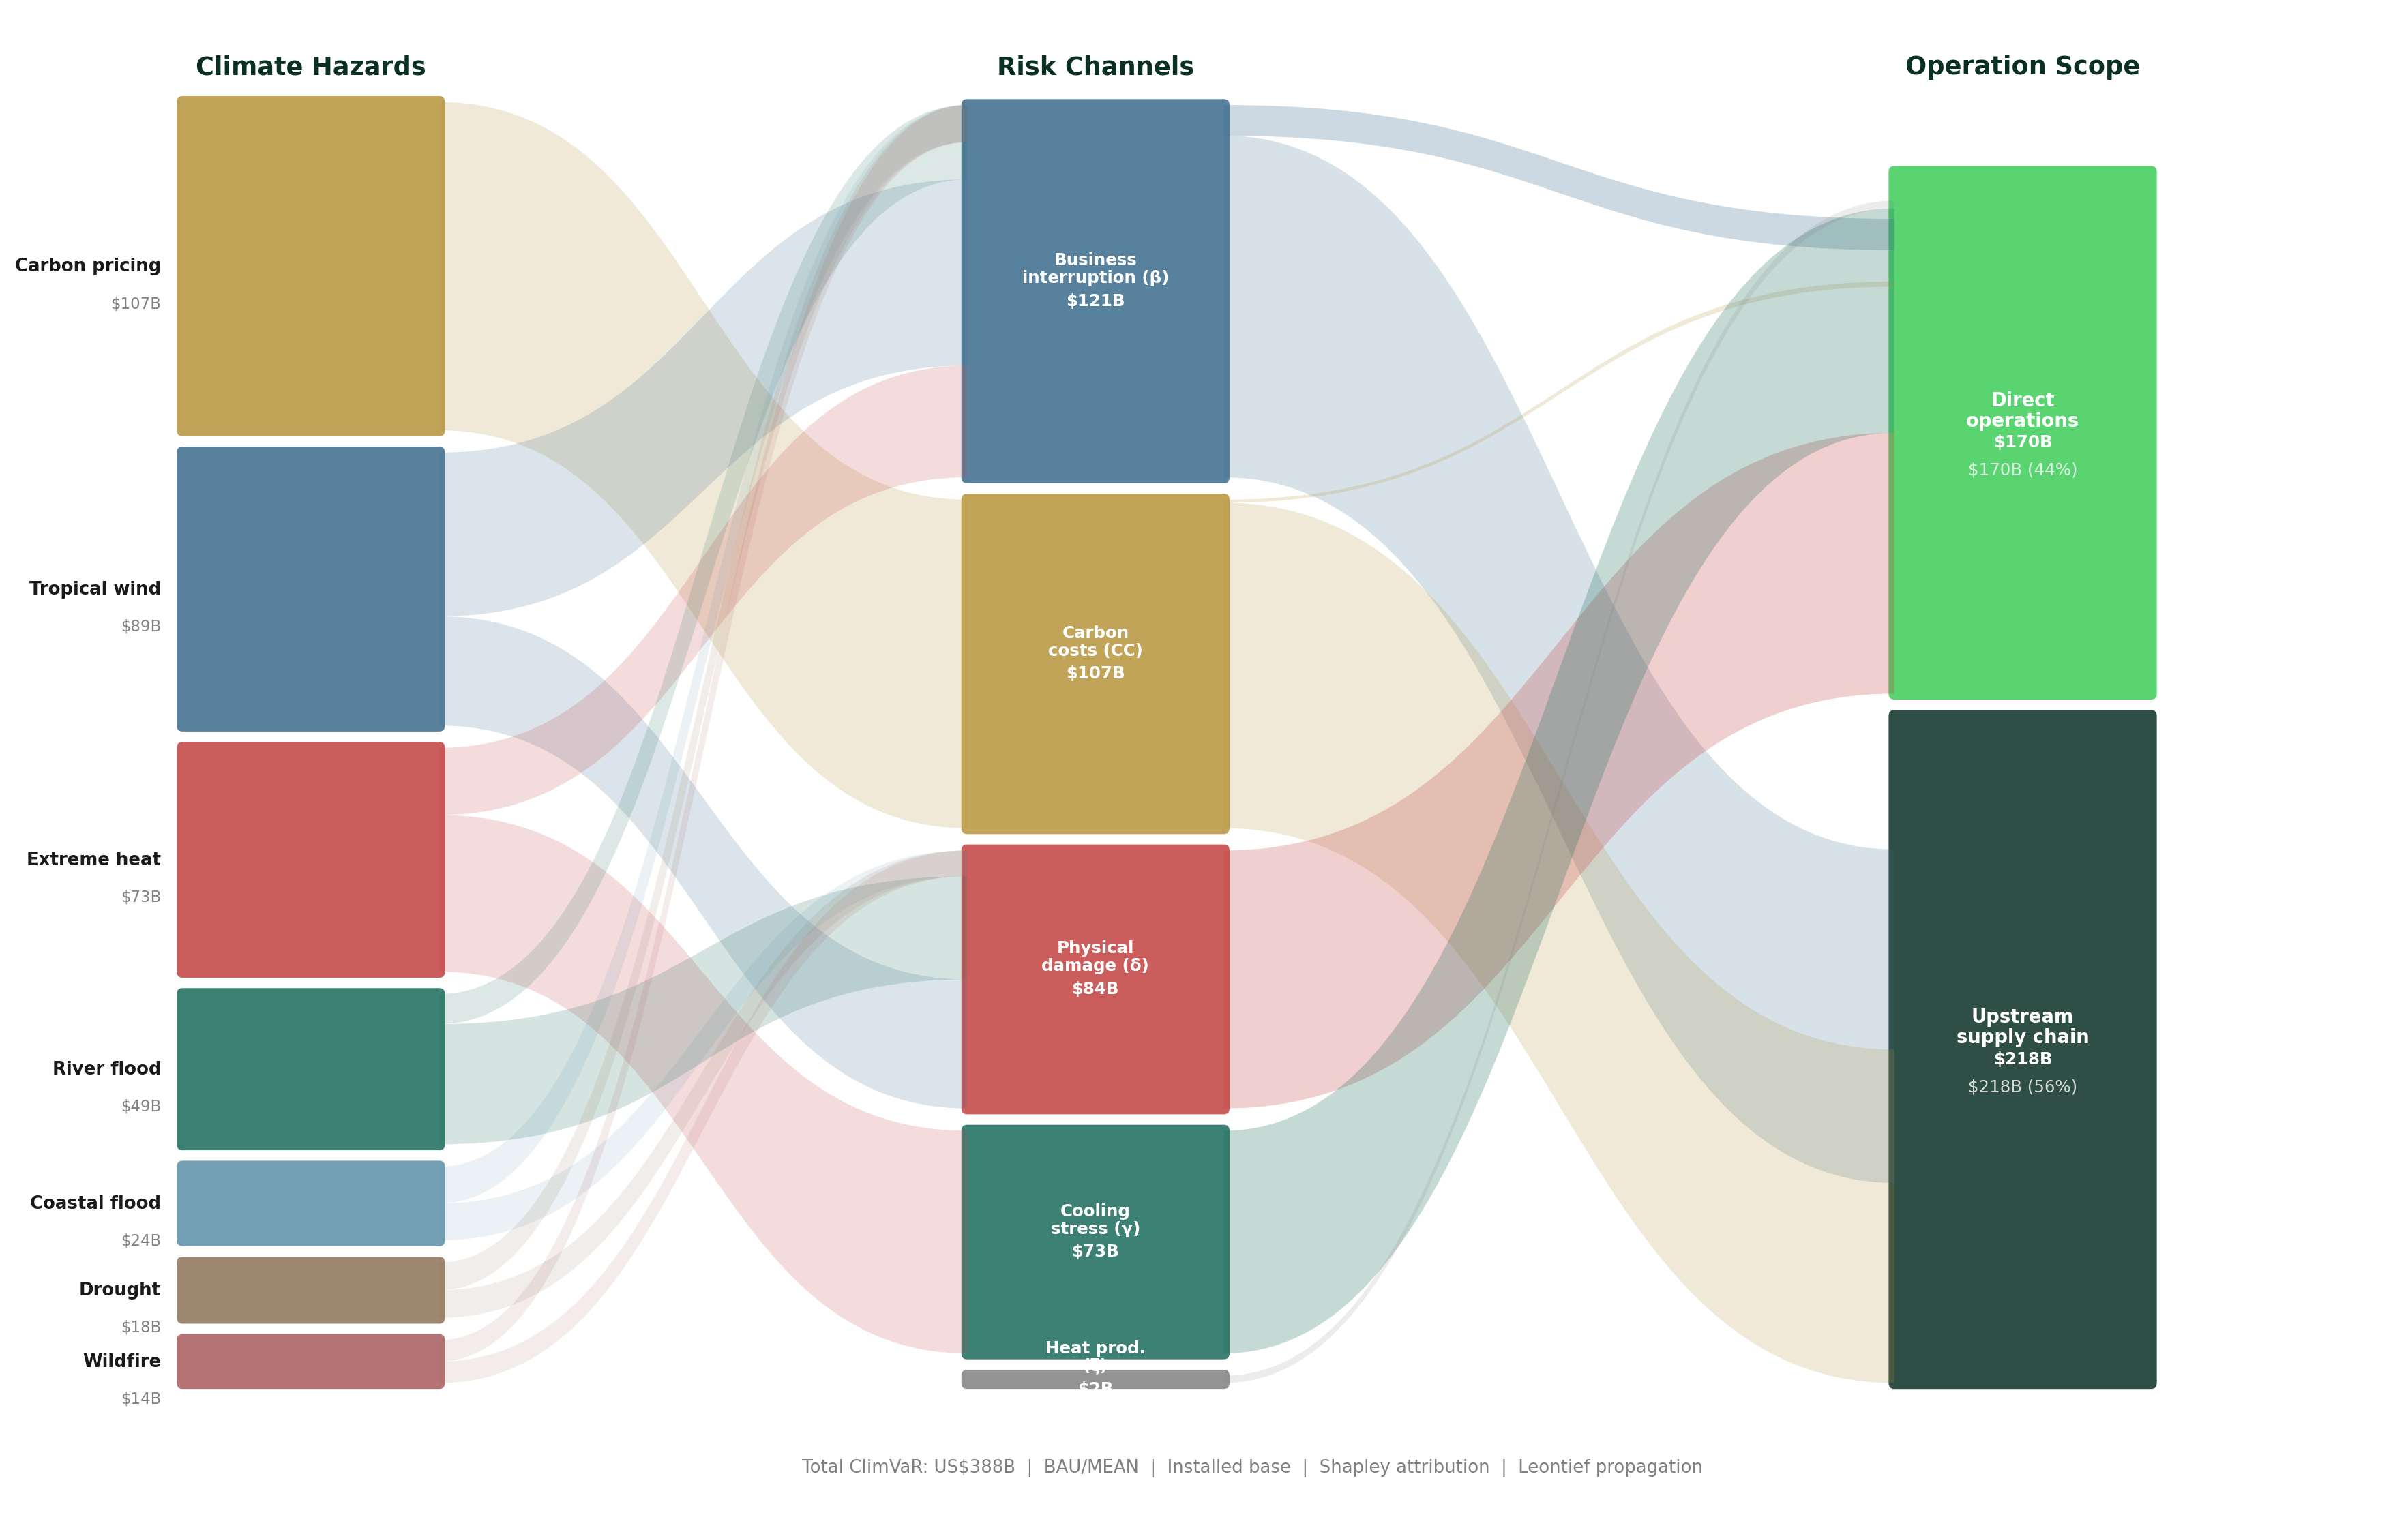
\includegraphics[width=\textwidth]{images/Image2.png}
\end{center}
\exhibitsource{Seven hazards propagate through four risk channels to erode US\$388B. Ribbon width proportional to US\$ value. Shapley attribution for hazard-to-channel mapping. BAU/MEAN, installed base.}

\begin{twocolbody}

\noindent Exhibit~11 maps the transmission mechanism from climate hazard to financial loss. On the left, seven physical hazards---ranked by dollar impact. Tropical wind (\$89B) dominates, followed by extreme heat (\$73B) and river flood (\$49B). Carbon pricing (\$107B) enters as a transition hazard, distinct from the physical channels.

Why does tropical wind rank first, ahead of flood? The answer is geographic spread. River flood inflicts severe damage at exposed sites but affects only the subset of facilities in floodplains. Tropical wind, by contrast, propagates through supply chains that serve the entire global portfolio: a typhoon disrupting semiconductor fabrication in Taiwan or power transformer production in coastal China degrades every facility that depends on those inputs, regardless of location. At the portfolio level, a hazard that touches many facilities indirectly outweighs one that devastates a few directly.

On the right, four risk channels aggregate these hazards into enterprise value loss. Business interruption (\$121B, 31\%) is the largest channel---but 91\% of it propagates through supply chains, not through direct facility damage. Carbon pricing (\$107B, 28\%) is almost entirely Scope~2: grid carbon intensity, not on-site emissions. Physical damage (\$84B, 22\%) concentrates in flood-exposed regions. Cooling stress (\$73B, 19\%) is the most geographically dispersed channel, affecting every facility where ambient temperature is rising.

The ribbons connecting hazards to channels show that a single hazard can affect multiple channels simultaneously. Tropical wind drives both business interruption (through supply chain disruption) and physical damage (through structural impact). Extreme heat drives both cooling stress (through energy costs) and business interruption (through grid overload). This non-additivity is precisely why the Shapley decomposition is required: simple allocation rules would either double-count or undercount hazard contributions.

\end{twocolbody}

% ==============================================================================
% FINDING 1
% ==============================================================================
\clearpage\thispagestyle{chapterstart}

\subsection*{Finding 1: Aggregate Exposure}
\sectionsubtitle{Climate risks on direct operations, but also upstream supply chain}
\greensep

\begin{twocolbody}

\noindent The \$388~billion headline figure on the installed base is not a single uniform risk. Exhibit~12 decomposes it into five channels, each with distinct drivers and distinct adaptation levers. The most consequential finding at this level is the dominance of supply chain propagation: business interruption alone accounts for \$121B, of which 91\% originates upstream. Operators monitoring only on-site hazards miss the primary risk vector.

\end{twocolbody}

\vspace{2mm}
\exhibitcaption{12}{ClimVaR decomposition by risk channel---installed base, BAU/MEAN.}

\begin{center}
\datatablesetup
\begin{tabularx}{\textwidth}{>{\raggedright\arraybackslash}p{4cm} >{\raggedleft\arraybackslash}X >{\raggedleft\arraybackslash}X >{\raggedright\arraybackslash}X}
\toprule
\datatableheader
\thd{Risk Channel} & \thd{Impact (\$B)} & \thd{Share} & \thd{Mechanism} \\
\midrule
Business interruption ($\beta$) & 121.4 & 31\% & Extreme events, grid stress, downtime \\
Carbon costs (CC$^{1,2,3}$) & 107.1 & 28\% & Grid emissions $\times$ carbon price trajectory \\
Physical damages ($\delta$) & 84.1 & 22\% & Structural damage from floods, storms \\
Cooling penalty ($\gamma$) & 72.6 & 19\% & Rising ambient temperature $\to$ energy cost \\
Heat productivity ($\xi$) & 2.4 & 1\% & Worker and equipment efficiency losses \\
\midrule
\textbf{Total ClimVaR} & \textbf{387.5} & \textbf{100\%} & \\
\bottomrule
\end{tabularx}
\datatableclear
\end{center}

\begin{twocolbody}

\noindent The physical risk channels (business interruption + damages + cooling) account for 72\% of total ClimVaR on the installed base. Carbon costs represent 28\%---a ratio that inverts sharply when AI infrastructure is added (Finding~4).

The channel decomposition disaggregates further. Supply chain business interruption (\$111B) exceeds direct business interruption (\$10B) by a factor of eleven---the Leontief propagation channel dominates the interruption risk. Carbon costs are almost entirely Scope~2 (\$106B of \$107B), confirming that grid carbon intensity and PPA strategy are the primary levers for transition risk.

A further dimension is omitted from the current perimeter but warrants acknowledgment: nature-related risk. Water stress, biodiversity constraints on siting permits, and ecosystem degradation around cooling water sources are not captured in the five channels modeled here. Their inclusion would widen, not narrow, the exposure estimate.

\end{twocolbody}

\begin{tcolorbox}[colback=SEDarkGreen!5, colframe=SEGreen, title={\textcolor{SEGreen}{\textbf{Future Research}}}, fonttitle=\sffamily\bfseries]
\small
\textbf{Supply chain structural risk.} The current framework captures supply chain propagation via static Leontief coefficients. Future work should model dynamic rerouting under stress, concentration risk in critical components (advanced semiconductors, high-bandwidth memory, large power transformers), and the cascading effects of simultaneous disruptions across correlated supply nodes.

\textbf{Digital twin integration.} Coupling the ClimVaR model with facility-level digital twins would enable real-time scenario analysis: testing the financial impact of specific cooling system upgrades, backup power configurations, or supply chain diversification strategies before committing capital.
\end{tcolorbox}

\statcallout{US\$388 billion}{Climate Value at Risk on 8,572 installed data centers\\38.3\% of enterprise value --- BAU/MEAN pathway}

\exhibitcaption{13}{US\$388 billion decomposed by risk channel and region.}
\begin{center}
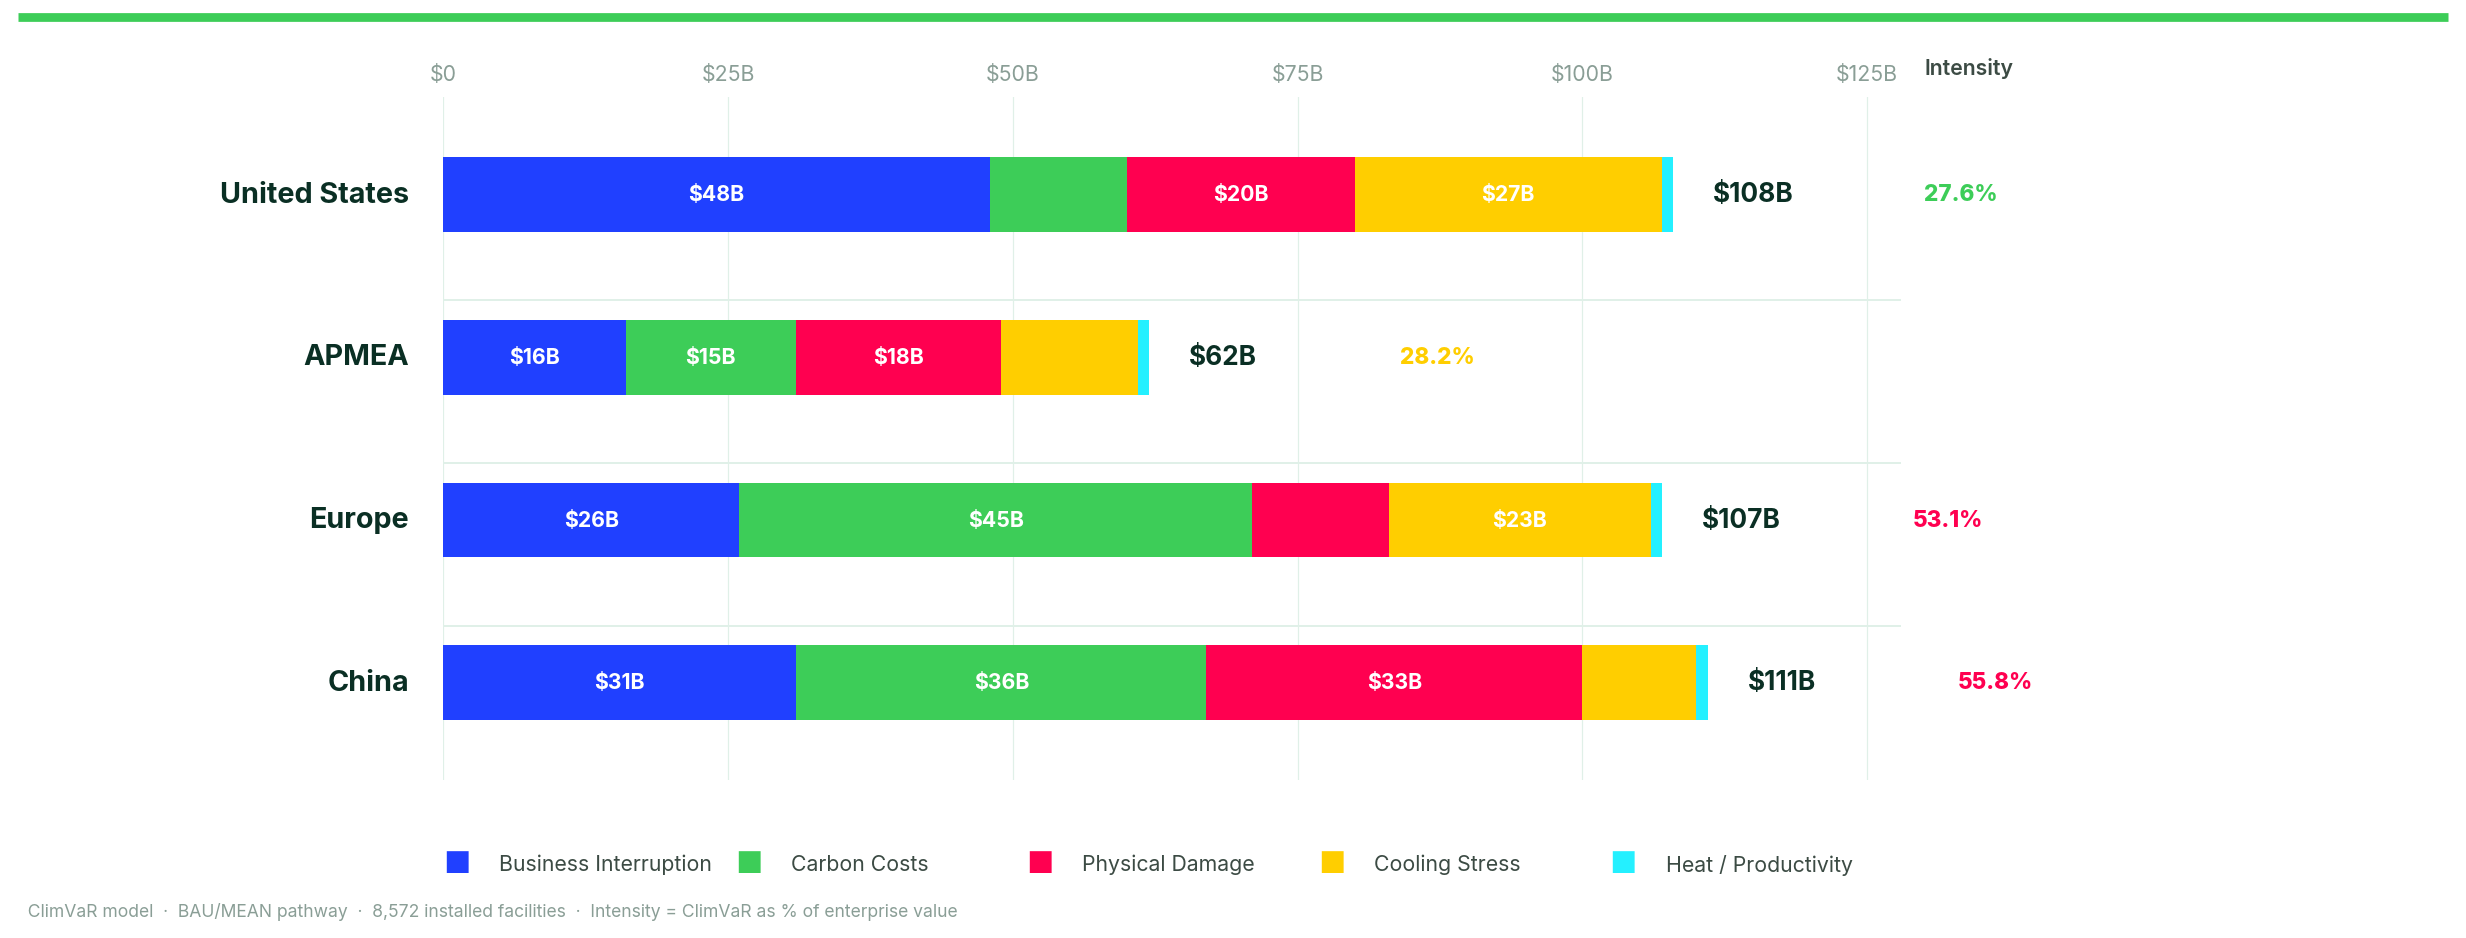
\includegraphics[width=\textwidth]{images/Image7.png}
\end{center}
\exhibitsource{Nested treemap: area proportional to ClimVaR in US\$B. Outer rectangles = regions; inner rectangles = risk channels. BAU/MEAN, installed base.}

% ==============================================================================
% FINDING 2
% ==============================================================================
\clearpage\thispagestyle{chapterstart}

\subsection*{Finding 2: Geographic Dispersion}
\sectionsubtitle{Each geography comes with its own risks}
\greensep

\vspace{2mm}
\exhibitcaption{14}{ClimVaR by region---installed base, BAU/MEAN pathway.}

\begin{center}
\datatablesetup
\begin{tabularx}{\textwidth}{l >{\raggedleft\arraybackslash}X >{\raggedleft\arraybackslash}X >{\raggedleft\arraybackslash}X >{\raggedleft\arraybackslash}X >{\raggedleft\arraybackslash}X >{\raggedleft\arraybackslash}X >{\raggedleft\arraybackslash}X}
\toprule
\datatableheader
\thd{Region} & \thd{V$_0$ (\$B)} & \thd{BI} & \thd{Cooling} & \thd{Damages} & \thd{Carbon} & \thd{ClimVaR (\$B)} & \thd{Intensity} \\
\midrule
United States & 393 & 48 & 27 & 20 & 12 & 108 & 27.6\% \\
APMEA & 220 & 16 & 12 & 18 & 15 & 62 & 28.2\% \\
Europe & 201 & 26 & 23 & 12 & 45 & 107 & 53.1\% \\
China & 198 & 31 & 10 & 33 & 36 & 111 & 55.8\% \\
\midrule
\textbf{Global} & \textbf{1,012} & \textbf{121} & \textbf{73} & \textbf{84} & \textbf{107} & \textbf{388} & \textbf{38.3\%} \\
\bottomrule
\end{tabularx}
\datatableclear
\end{center}

\begin{twocolbody}

\noindent The range from 27.6\% (US) to 55.8\% (China) represents a $2\times$ dispersion factor. Two facilities of identical design, operated by the same company, applying the same standards, face substantially different climate-adjusted valuations depending on where they sit.

The aggregate percentage does not determine adaptation strategy: what matters is \textit{which channels} drive the exposure. Each region carries a distinct channel fingerprint. In the United States, business interruption dominates (44\% of regional ClimVaR), driven by supply chain concentration and grid stress. In Europe, carbon costs lead (43\%), reflecting higher carbon prices and grid emission intensity. In Asia-Pacific, physical damage is the largest channel (39\%), driven by tropical cyclone and flood exposure. China carries a dual profile: carbon costs (33\%) and physical damages (30\%) compound.

\end{twocolbody}

\begin{pullquote}
Treating ``data center climate risk'' as a single global category hides a twofold dispersion in intensity and different levers in each market. A uniform adaptation strategy systematically underinvests in the dominant channel.
\end{pullquote}

\exhibitcaption{15}{Regional channel fingerprints: same global risk, different local drivers.}
\begin{center}
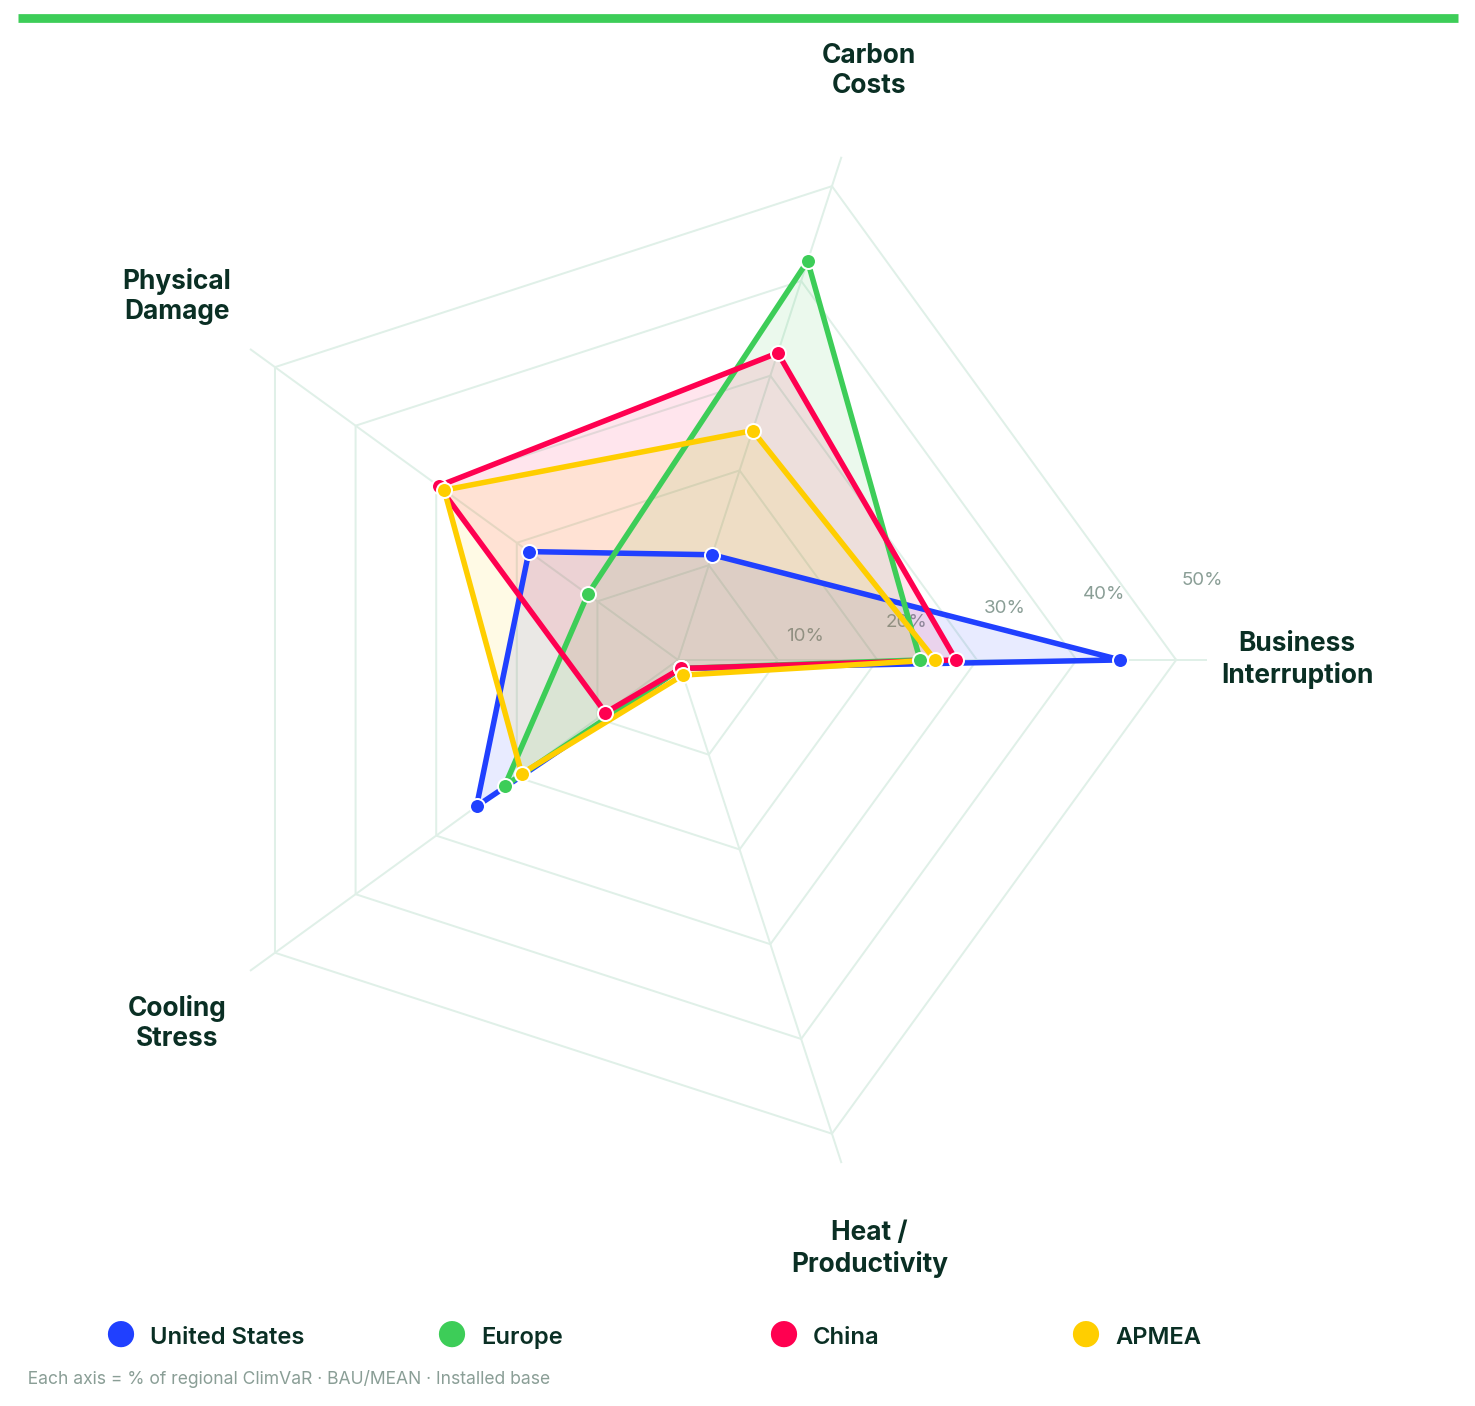
\includegraphics[width=\textwidth]{images/Image4.png}
\end{center}
\exhibitsource{Radar chart: each polygon is one region's channel fingerprint (\% of regional ClimVaR). The asymmetry between shapes shows why a uniform adaptation strategy fails.}

% ==============================================================================
% FINDING 3 (was Finding 4 — swapped per Thomas)
% ==============================================================================
\clearpage\thispagestyle{chapterstart}

\subsection*{Finding 3: Adaptation Value}
\sectionsubtitle{Net adaptation reduces exposure by 30--39\%, with positive returns}
\greensep

\vspace{2mm}
\exhibitcaption{16}{Adaptation value creation---installed base, BAU/MEAN pathway.}

\begin{center}
\datatablesetup
\begin{tabularx}{\textwidth}{l >{\raggedleft\arraybackslash}X >{\raggedleft\arraybackslash}X >{\raggedleft\arraybackslash}X >{\raggedleft\arraybackslash}X >{\raggedleft\arraybackslash}X >{\raggedleft\arraybackslash}X}
\toprule
\datatableheader
\thd{Region} & \thd{CV Baseline} & \thd{CV Selective} & \thd{$\Delta$ Sel.} & \thd{CV Proactive} & \thd{$\Delta$ Proact.} & \thd{Reduction} \\
\midrule
US & 108 & 89 & 19 & 72 & 36 & 34\% \\
Europe & 107 & 81 & 26 & 60 & 46 & 43\% \\
APMEA & 62 & 49 & 13 & 39 & 23 & 37\% \\
China & 111 & 86 & 24 & 67 & 44 & 40\% \\
\midrule
\textbf{Global} & \textbf{388} & \textbf{305} & \textbf{83} & \textbf{238} & \textbf{150} & \textbf{39\%} \\
\bottomrule
\end{tabularx}
\datatableclear
\end{center}

\begin{twocolbody}

\noindent The value of adaptation scales with portfolio size. Under AWB, Proactive protects \$1,063B of value; Selective alone protects \$609B.

Two investment logics emerge. \textbf{Selective}---adapting only new builds---captures 56\% of Proactive's value at 15--20\% of the capital outlay. It targets the highest-return interventions: PPAs on new builds, liquid cooling at design stage, climate-aware siting. \textbf{Proactive} adds value through legacy retrofit, structured adaptation programs, and portfolio-level geographic rebalancing---measures that are more expensive per unit of risk reduced but address the 60--70\% of installed capacity that will still operate through 2040.

Carbon is the most responsive channel ($-$63\% via PPAs), followed by cooling and business interruption (40--60\%). All reduction figures are \textbf{net}: they account for the capital and operating expenditure of each adaptation measure. PPA procurement generates an upfront CAPEX commitment but reduces OPEX (energy cost and carbon liability) over the contract lifetime; liquid cooling adds 10--15\% to facility CAPEX but lowers cooling OPEX by 30--40\% in hot climates. The temporal profile matters: most adaptation measures front-load capital expenditure in years 1--3 and deliver net OPEX savings from year 4 onward.

Adaptation value \textit{increases with climate policy ambition}. Under NZT/Proactive, aggregate ClimVaR drops by 53\% versus NZT/Baseline. Operators who invest today are hedged against the transition scenario where that investment pays the most.

\end{twocolbody}

\subsection*{}
\sectionsubtitle{Local adaptation can only go so far}
\greensep

\begin{twocolbody}

\noindent The residual 61\% of ClimVaR that Proactive adaptation cannot eliminate is not a shortcoming of the adaptation program---it reflects structural limits. Supply chain concentration in East Asia, thermodynamic ceilings on cooling efficiency, and the fixed geographic location of 8,572 existing facilities set a floor on facility-level risk reduction. Beyond this floor, further risk mitigation requires collective instruments: public risk-sharing mechanisms, infrastructure stress testing, and regulatory frameworks calibrated to actual financial exposure rather than reported emissions.

\end{twocolbody}

\vspace{3mm}
\begin{center}
\begin{minipage}[t]{0.3\textwidth}
  \metriccard[SEGreen]{BASELINE}{US\$388B}{No additional adaptation}
\end{minipage}\hfill
\begin{minipage}[t]{0.3\textwidth}
  \metriccard[SEWarmGold]{SELECTIVE}{US\$305B}{One champion action\\per facility}
\end{minipage}\hfill
\begin{minipage}[t]{0.3\textwidth}
  \metriccard[SEDarkGreen]{PROACTIVE}{US\$238B}{Comprehensive\\adaptation}
\end{minipage}
\end{center}

\exhibitcaption{17}{The adaptation effect: \$150 billion in protected value across all channels.}
\begin{center}
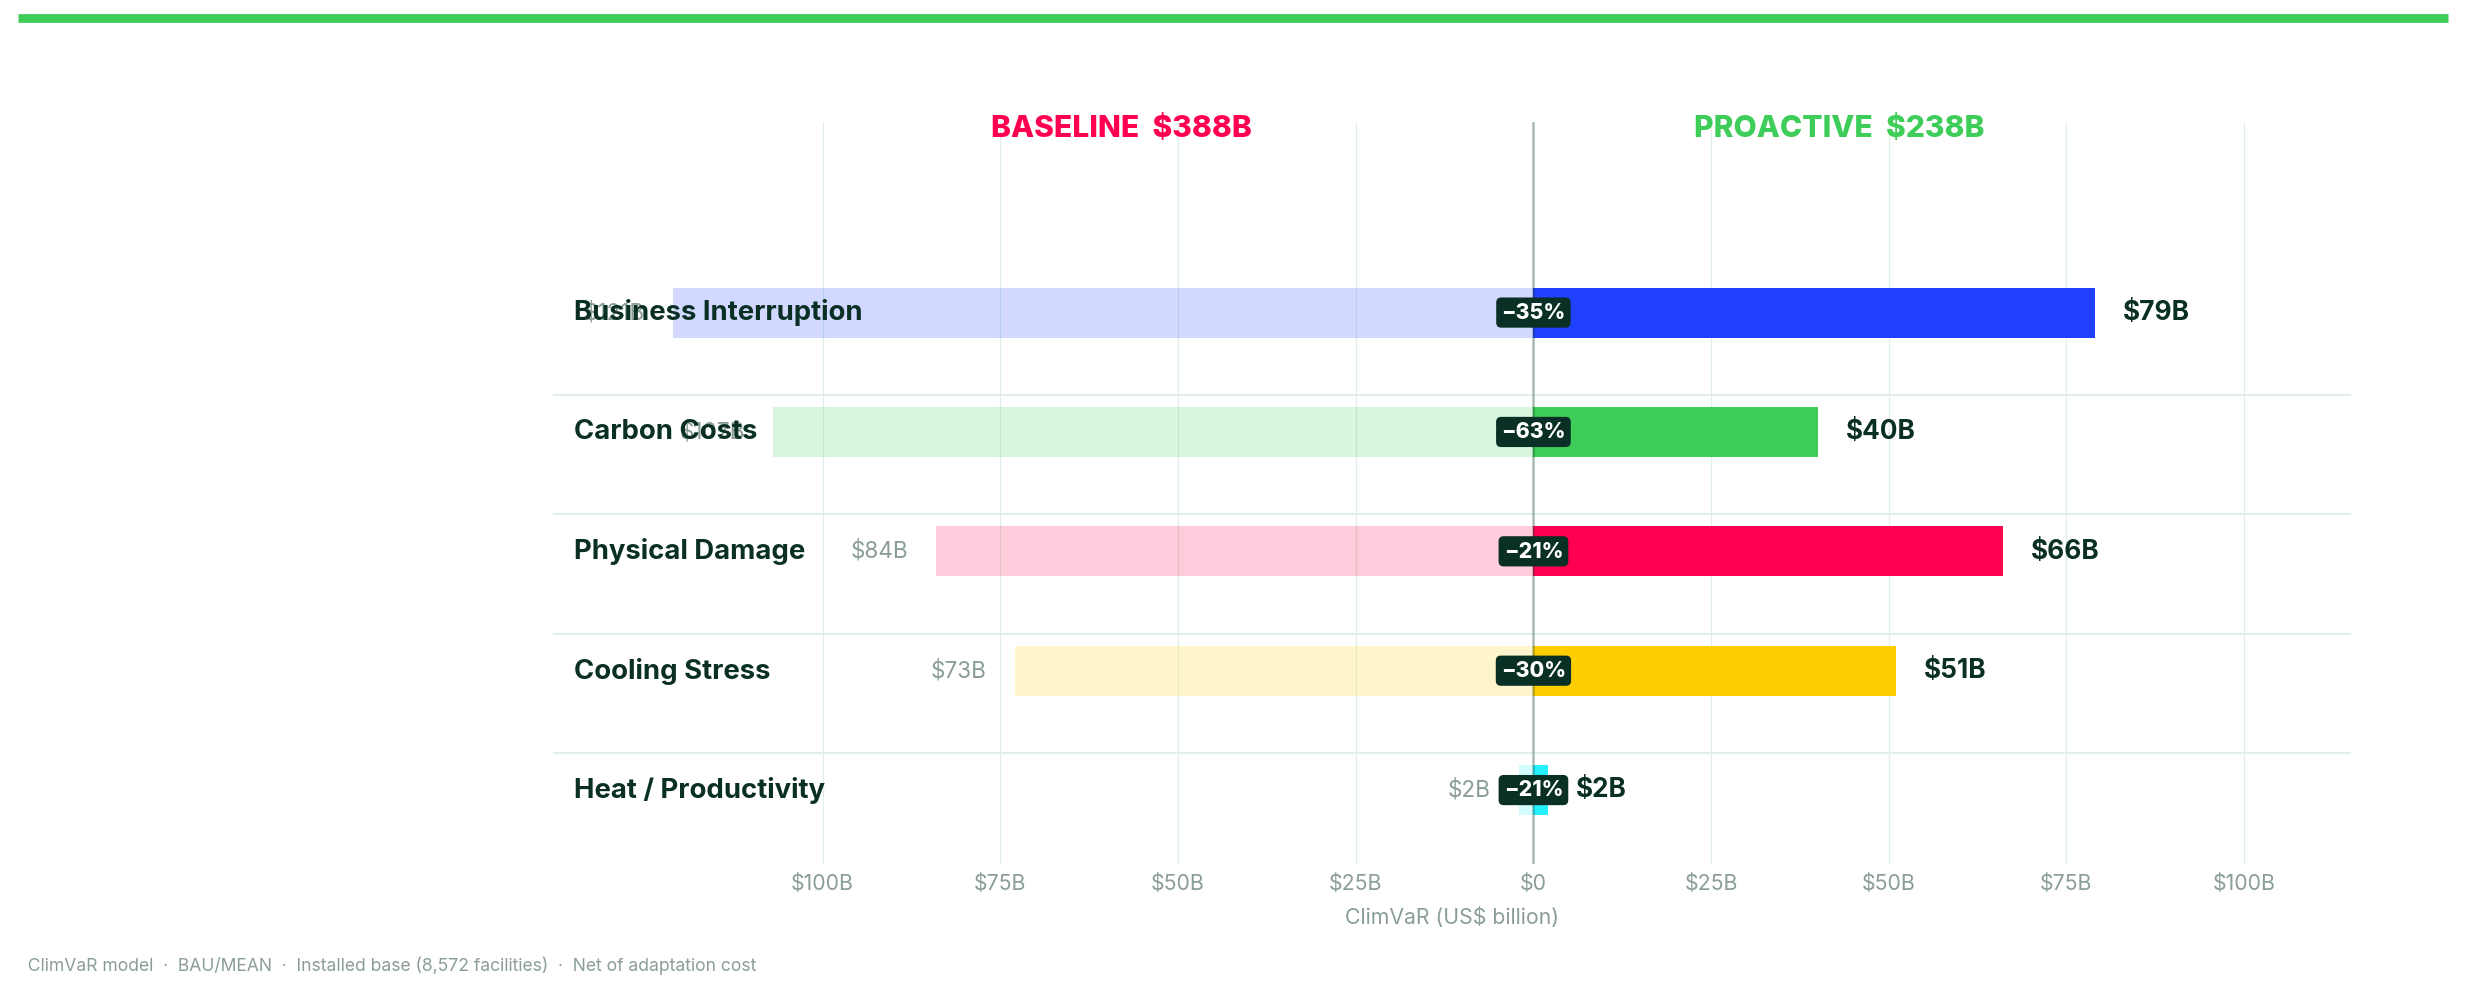
\includegraphics[width=\textwidth]{images/Image6.png}
\end{center}
\exhibitsource{Butterfly chart: left bars = Baseline (\$388B), right bars = Proactive (\$238B). Central badges show net reduction per channel. Same channel colors throughout.}

\exhibitcaption{18}{Channel-by-channel waterfall from Baseline to Proactive.}
\begin{center}
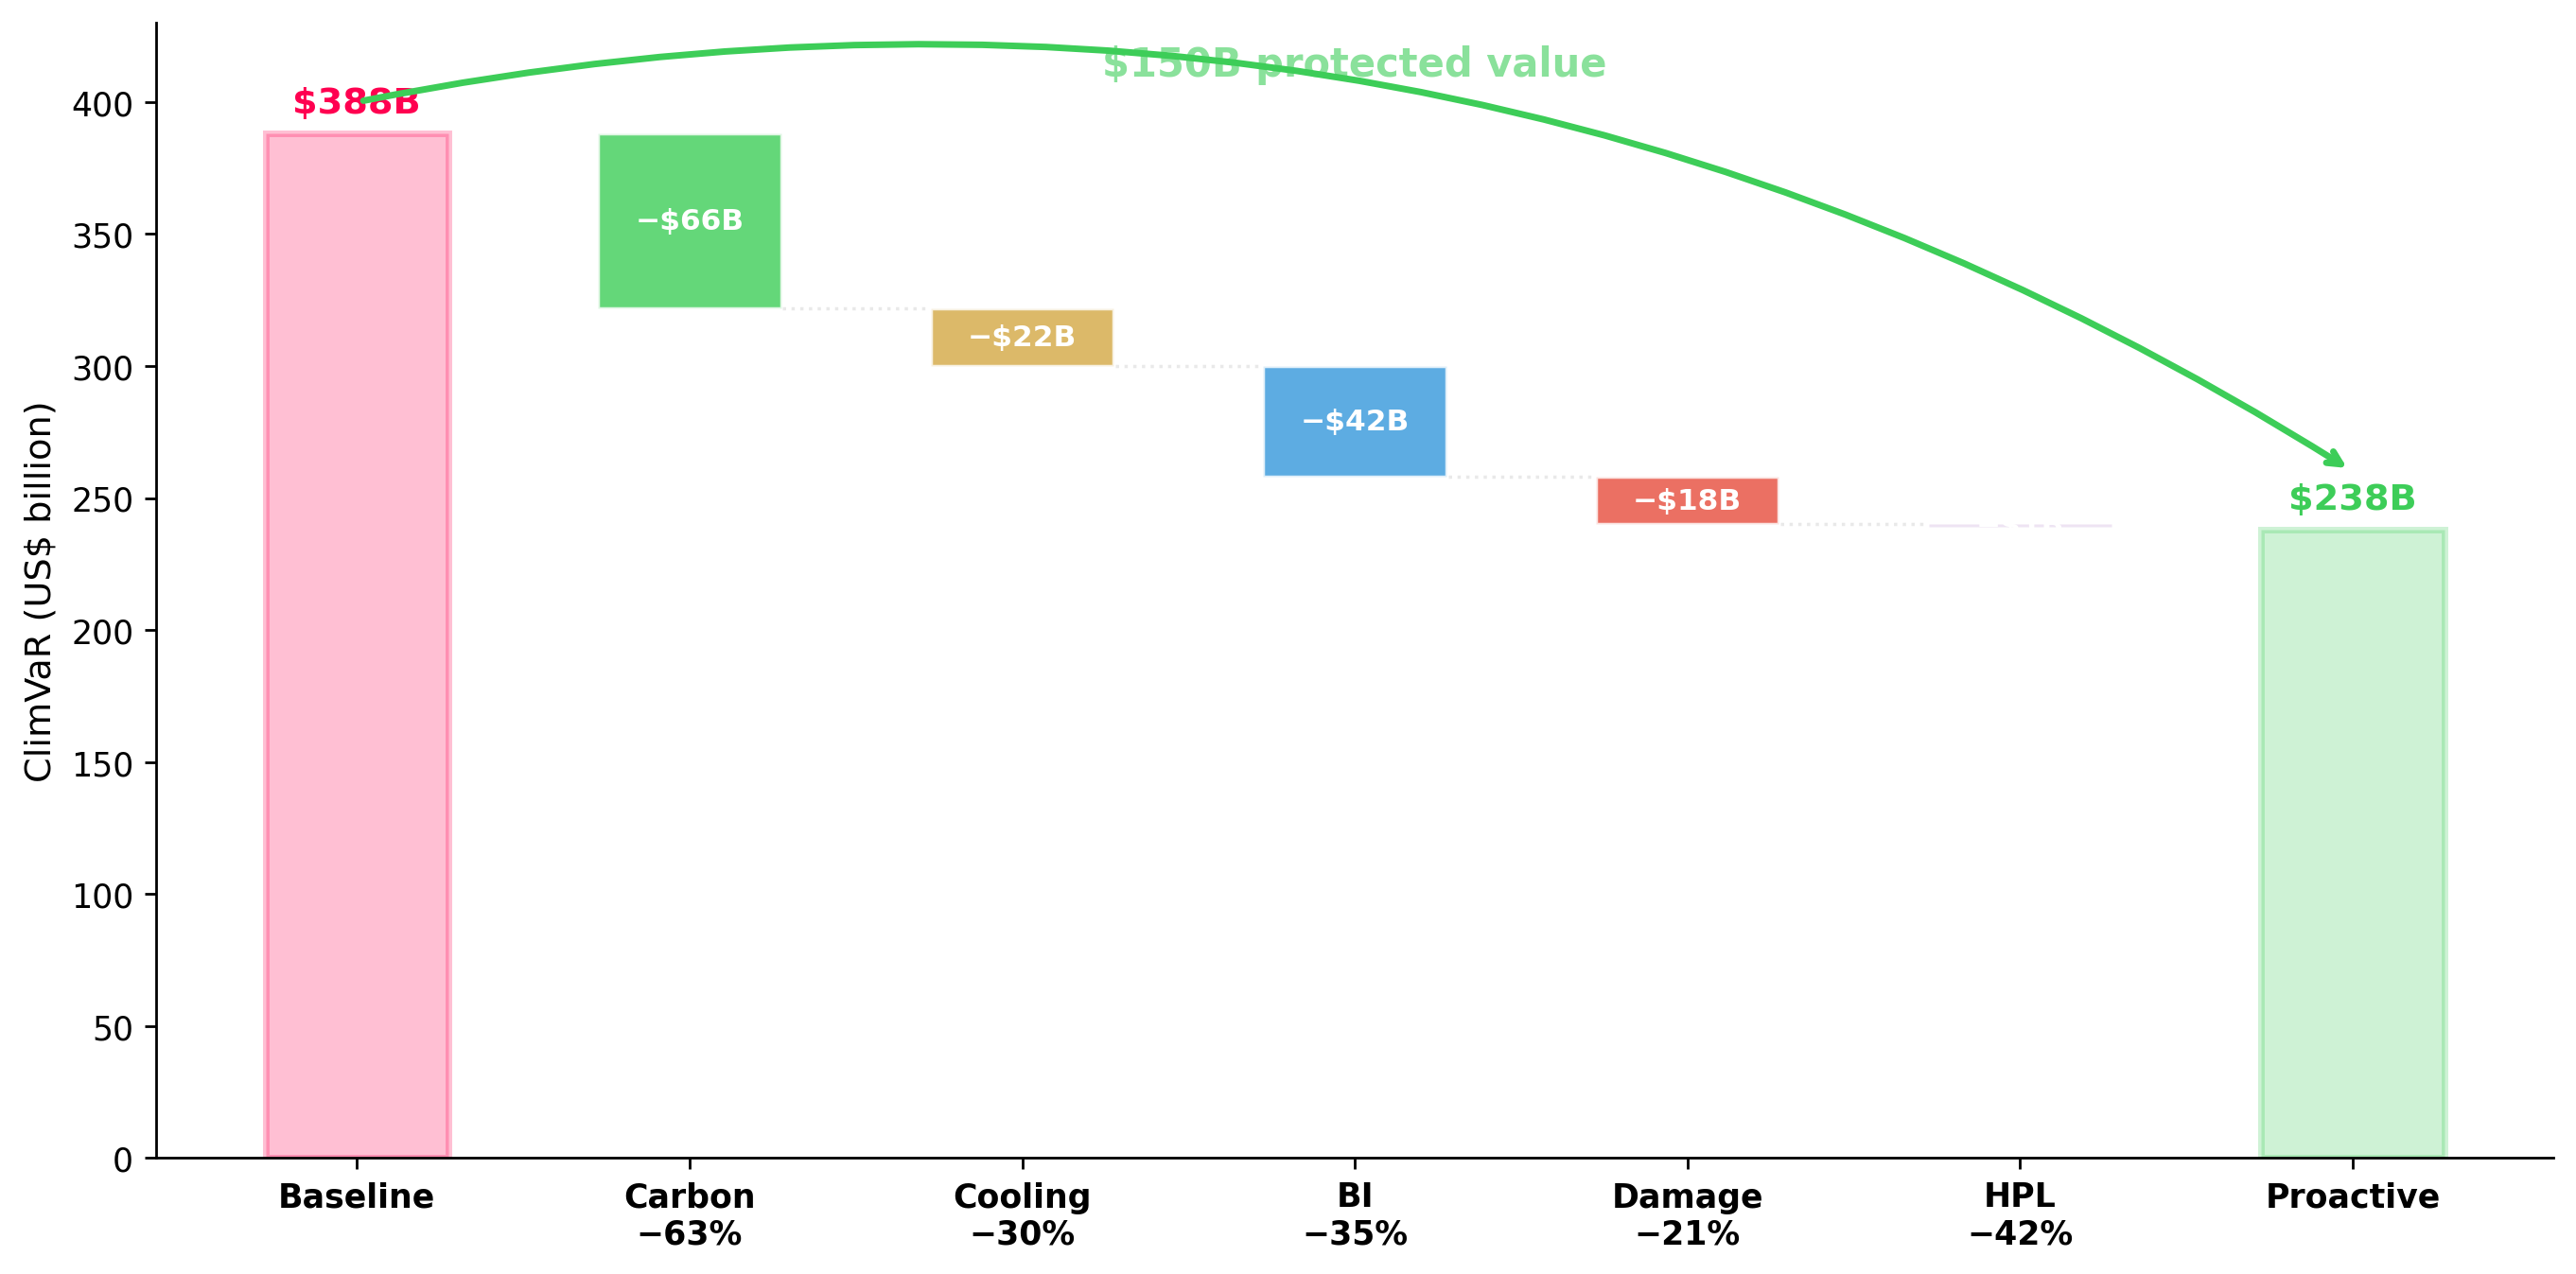
\includegraphics[width=\textwidth]{images/Image3.png}
\end{center}
\exhibitsource{Each step shows one channel's contribution to risk reduction. Carbon (\$66B, $-$63\%) is the most responsive via PPAs; physical damage (\$18B, $-$21\%) the least. The residual \$238B reflects exposure that facility-level action cannot eliminate.}

\exhibitcaption{19}{Marginal abatement cost of climate risk: 8 of 10 actions below break-even.}
\begin{center}
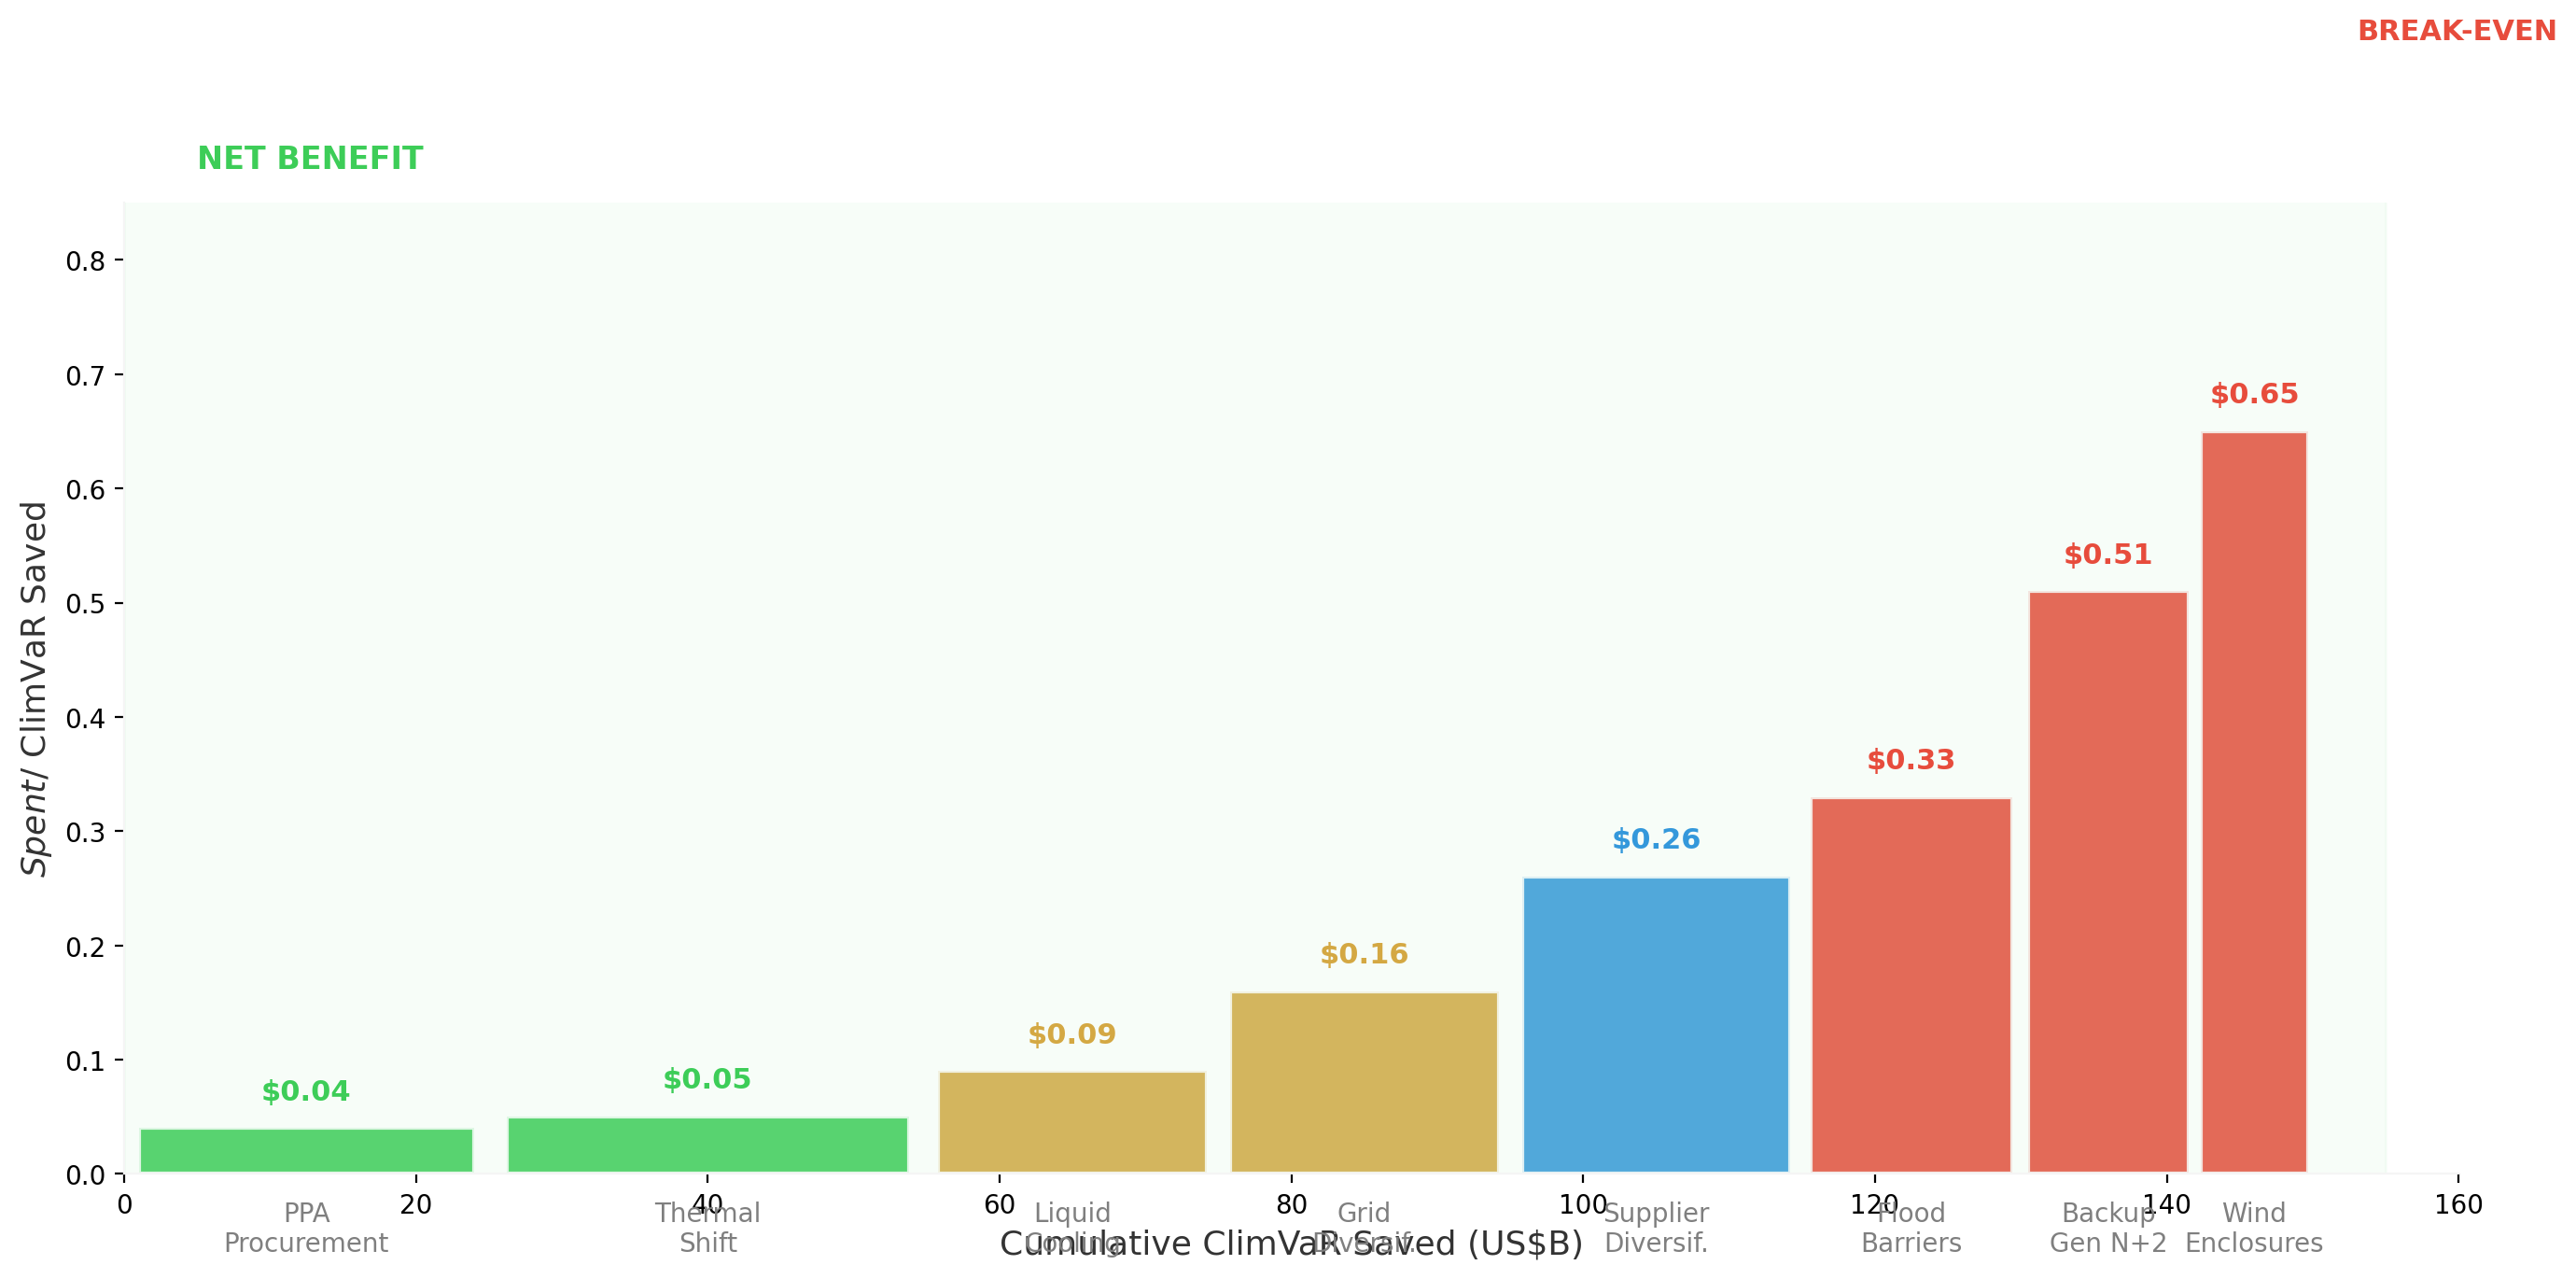
\includegraphics[width=\textwidth]{images/Image5a.png}
\end{center}
\exhibitsource{Horizontal axis: cumulative ClimVaR saved. Vertical: cost per dollar of risk saved. Actions below 1.0 generate net positive returns. PPAs are the cheapest lever (\$0.04 per dollar saved).}

\exhibitcaption{20}{Value at risk waterfall: from enterprise value through erosion to recovery.}
\begin{center}
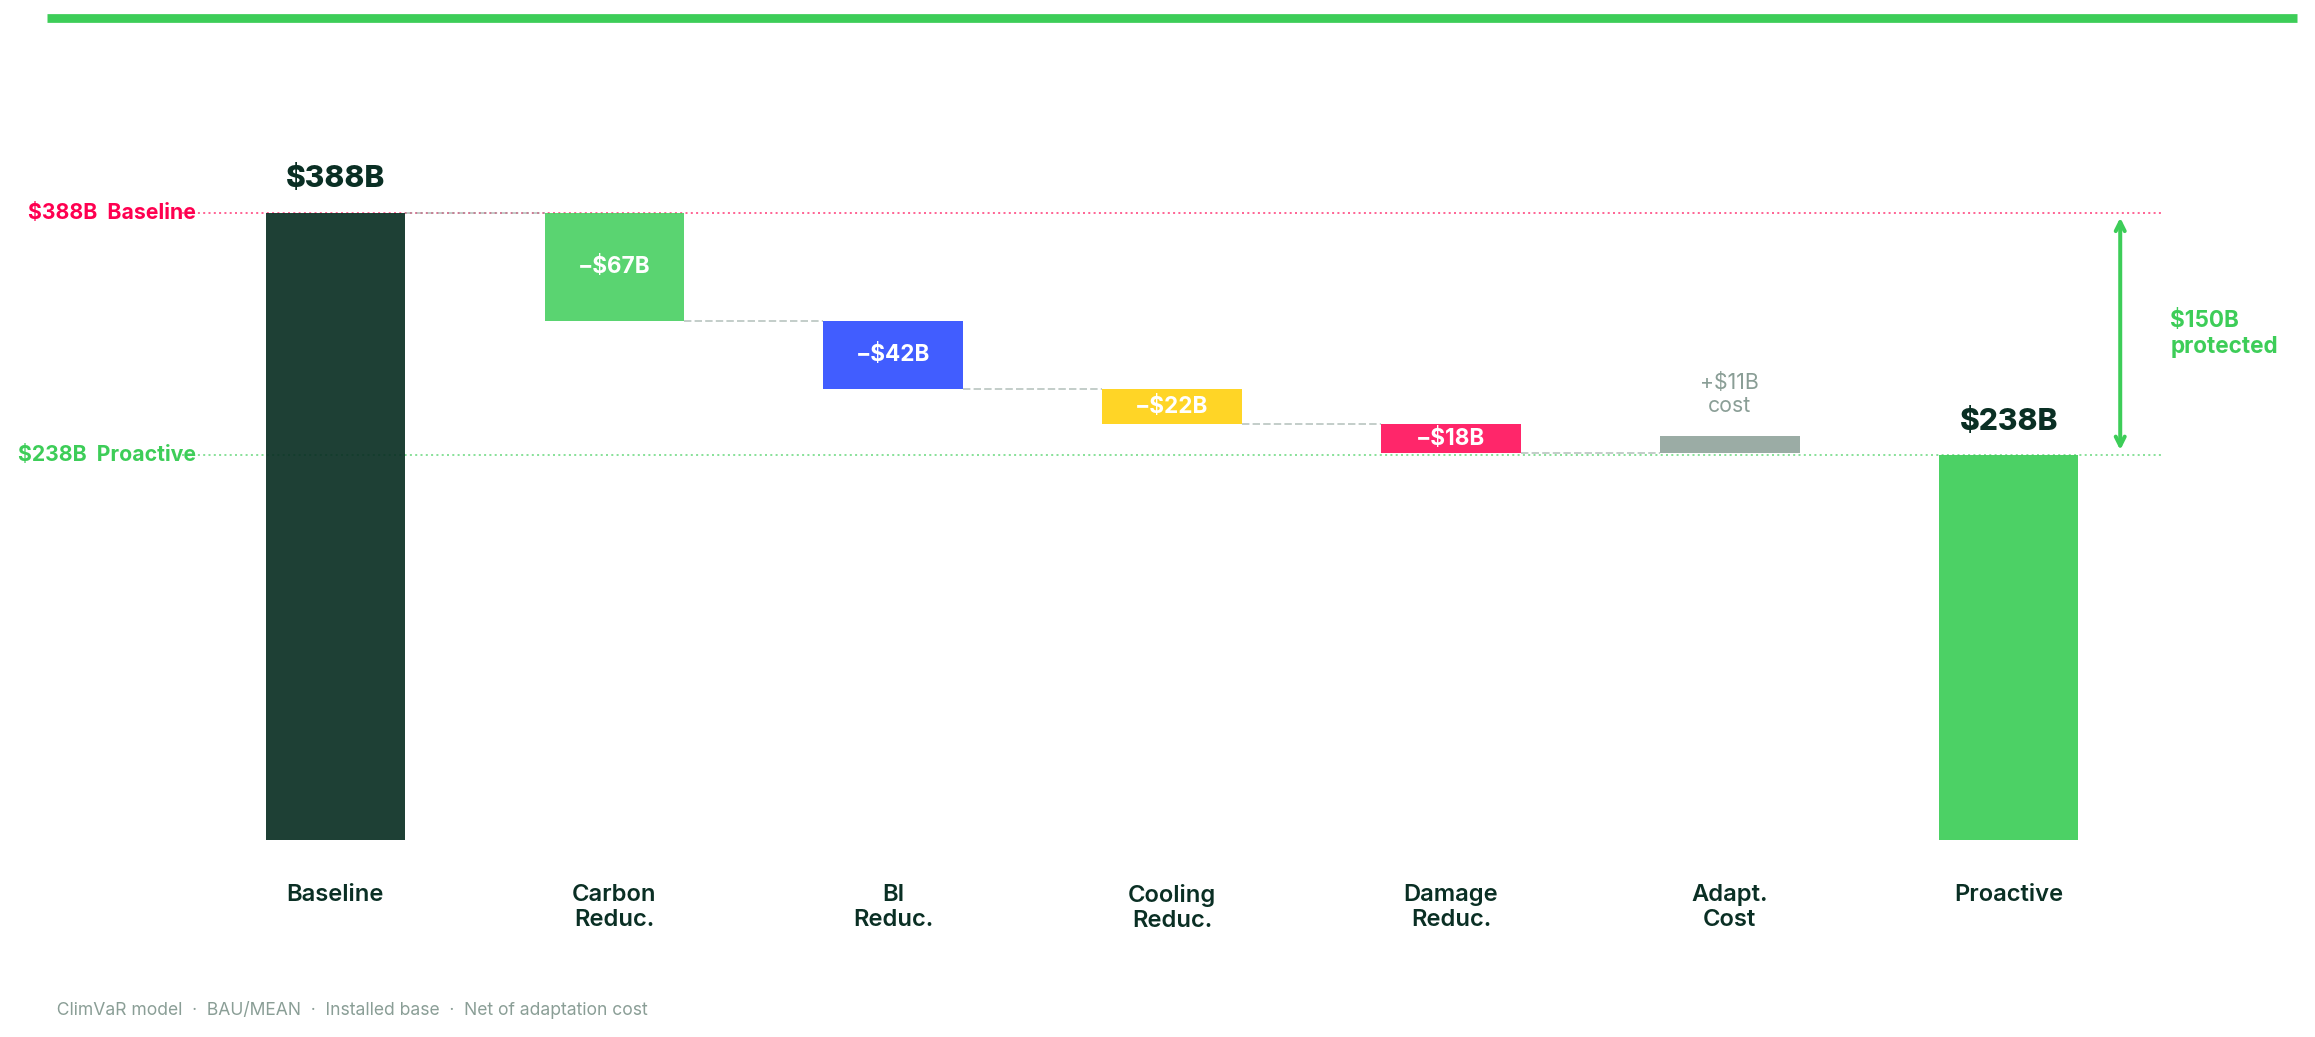
\includegraphics[width=\textwidth]{images/Image5b.png}
\end{center}
\exhibitsource{Dumbbell chart: hollow circles = Baseline, solid circles = Proactive. Line length proportional to adaptation value per channel. Carbon (−63\%) shows the longest travel; physical damage (−21\%) the shortest.}

% ==============================================================================
% FINDING 4 (was Finding 3 — swapped per Thomas)
% ==============================================================================
\clearpage\thispagestyle{chapterstart}

\subsection*{Finding 4: AI Amplification}
\sectionsubtitle{AI-era infrastructure carries $\times$2.6 the physical risk per GW}
\greensep

\begin{twocolbody}

\noindent The AI build-out does not replicate the risk profile of the installed base---it inverts it. On legacy facilities, carbon costs represent 28\% of total ClimVaR and physical channels 72\%. On AI-era facilities, physical channels account for 93--94\% while carbon drops to 6--7\%.

\end{twocolbody}

\vspace{2mm}
\exhibitcaption{21}{Channel decomposition: installed base versus AI-tier facilities (BAU/MEAN).}

\begin{center}
\datatablesetup
\begin{tabularx}{\textwidth}{>{\raggedright\arraybackslash}p{3.5cm} >{\raggedleft\arraybackslash}X >{\raggedleft\arraybackslash}X >{\raggedleft\arraybackslash}X >{\raggedleft\arraybackslash}X}
\toprule
\datatableheader
\thd{Channel} & \thd{Installed (\%)} & \thd{AI-LTG (\%)} & \thd{AI-SAI (\%)} & \thd{AI-AWB (\%)} \\
\midrule
Business Interruption & 31\% & 35\% & 33\% & 33\% \\
Physical Damages & 22\% & 29\% & 35\% & 36\% \\
Cooling & 19\% & 29\% & 25\% & 25\% \\
Carbon & 28\% & 7\% & 6\% & 6\% \\
Heat/Productivity & 1\% & 1\% & 1\% & 1\% \\
\midrule
\textbf{Physical (total)} & \textbf{72\%} & \textbf{93\%} & \textbf{94\%} & \textbf{94\%} \\
\bottomrule
\end{tabularx}
\datatableclear
\end{center}

\begin{twocolbody}

\noindent Three mechanisms drive the amplification. \textbf{Geographic concentration}: AI facilities cluster in regions combining cheap power with fast permitting---Texas, Virginia, parts of China and Southeast Asia---precisely the regions with elevated climate exposure. \textbf{Power density}: AI racks at 30--100+ kW generate more waste heat per square meter, making cooling failures more consequential. At a 5~kW/rack legacy facility, a cooling failure is an inconvenience; at a 60~kW/rack AI cluster, it triggers thermal shutdown within minutes. \textbf{Operational criticality}: AI training runs are non-interruptible workloads where interruption invalidates weeks of compute.

\textbf{A methodological note}: the $\times$2.6 factor combines two distinct components. The first is genuine physical amplification---higher power density, climate-exposed locations, concentrated supply chains. The second is a valuation effect: AI facilities carry higher asset value per MW (\$28--42M vs.\ \$9M for the installed base), which amplifies the \textit{financial} impact of identical physical hazards. Separating these two components matters for adaptation strategy: the physical component responds to engineering interventions; the valuation component responds to financial structuring and insurance design.

The implication for climate strategy is direct. Net-zero commitments---which address the carbon component through PPAs and grid decarbonization---are necessary for the installed base but insufficient for AI infrastructure. Under Net Zero Transition, installed base ClimVaR drops by 32\%, but AI-era ClimVaR drops by only 12--18\%, because the residual physical risk is irreducible through decarbonization alone. Under NZT, installed base ClimVaR paradoxically \textit{rises} from \$388B to \$845B (83\%), because higher carbon prices amplify the CC channel before physical adaptation takes effect. This counter-intuitive result means that operators relying on transition-only strategies---PPAs, grid decarbonization, Scope~2 reduction---face increasing, not decreasing, total exposure under ambitious climate policy.

\end{twocolbody}

\exhibitcaption{22}{Six futures for digital infrastructure: ClimVaR trajectories 2026--2050.}
\begin{center}
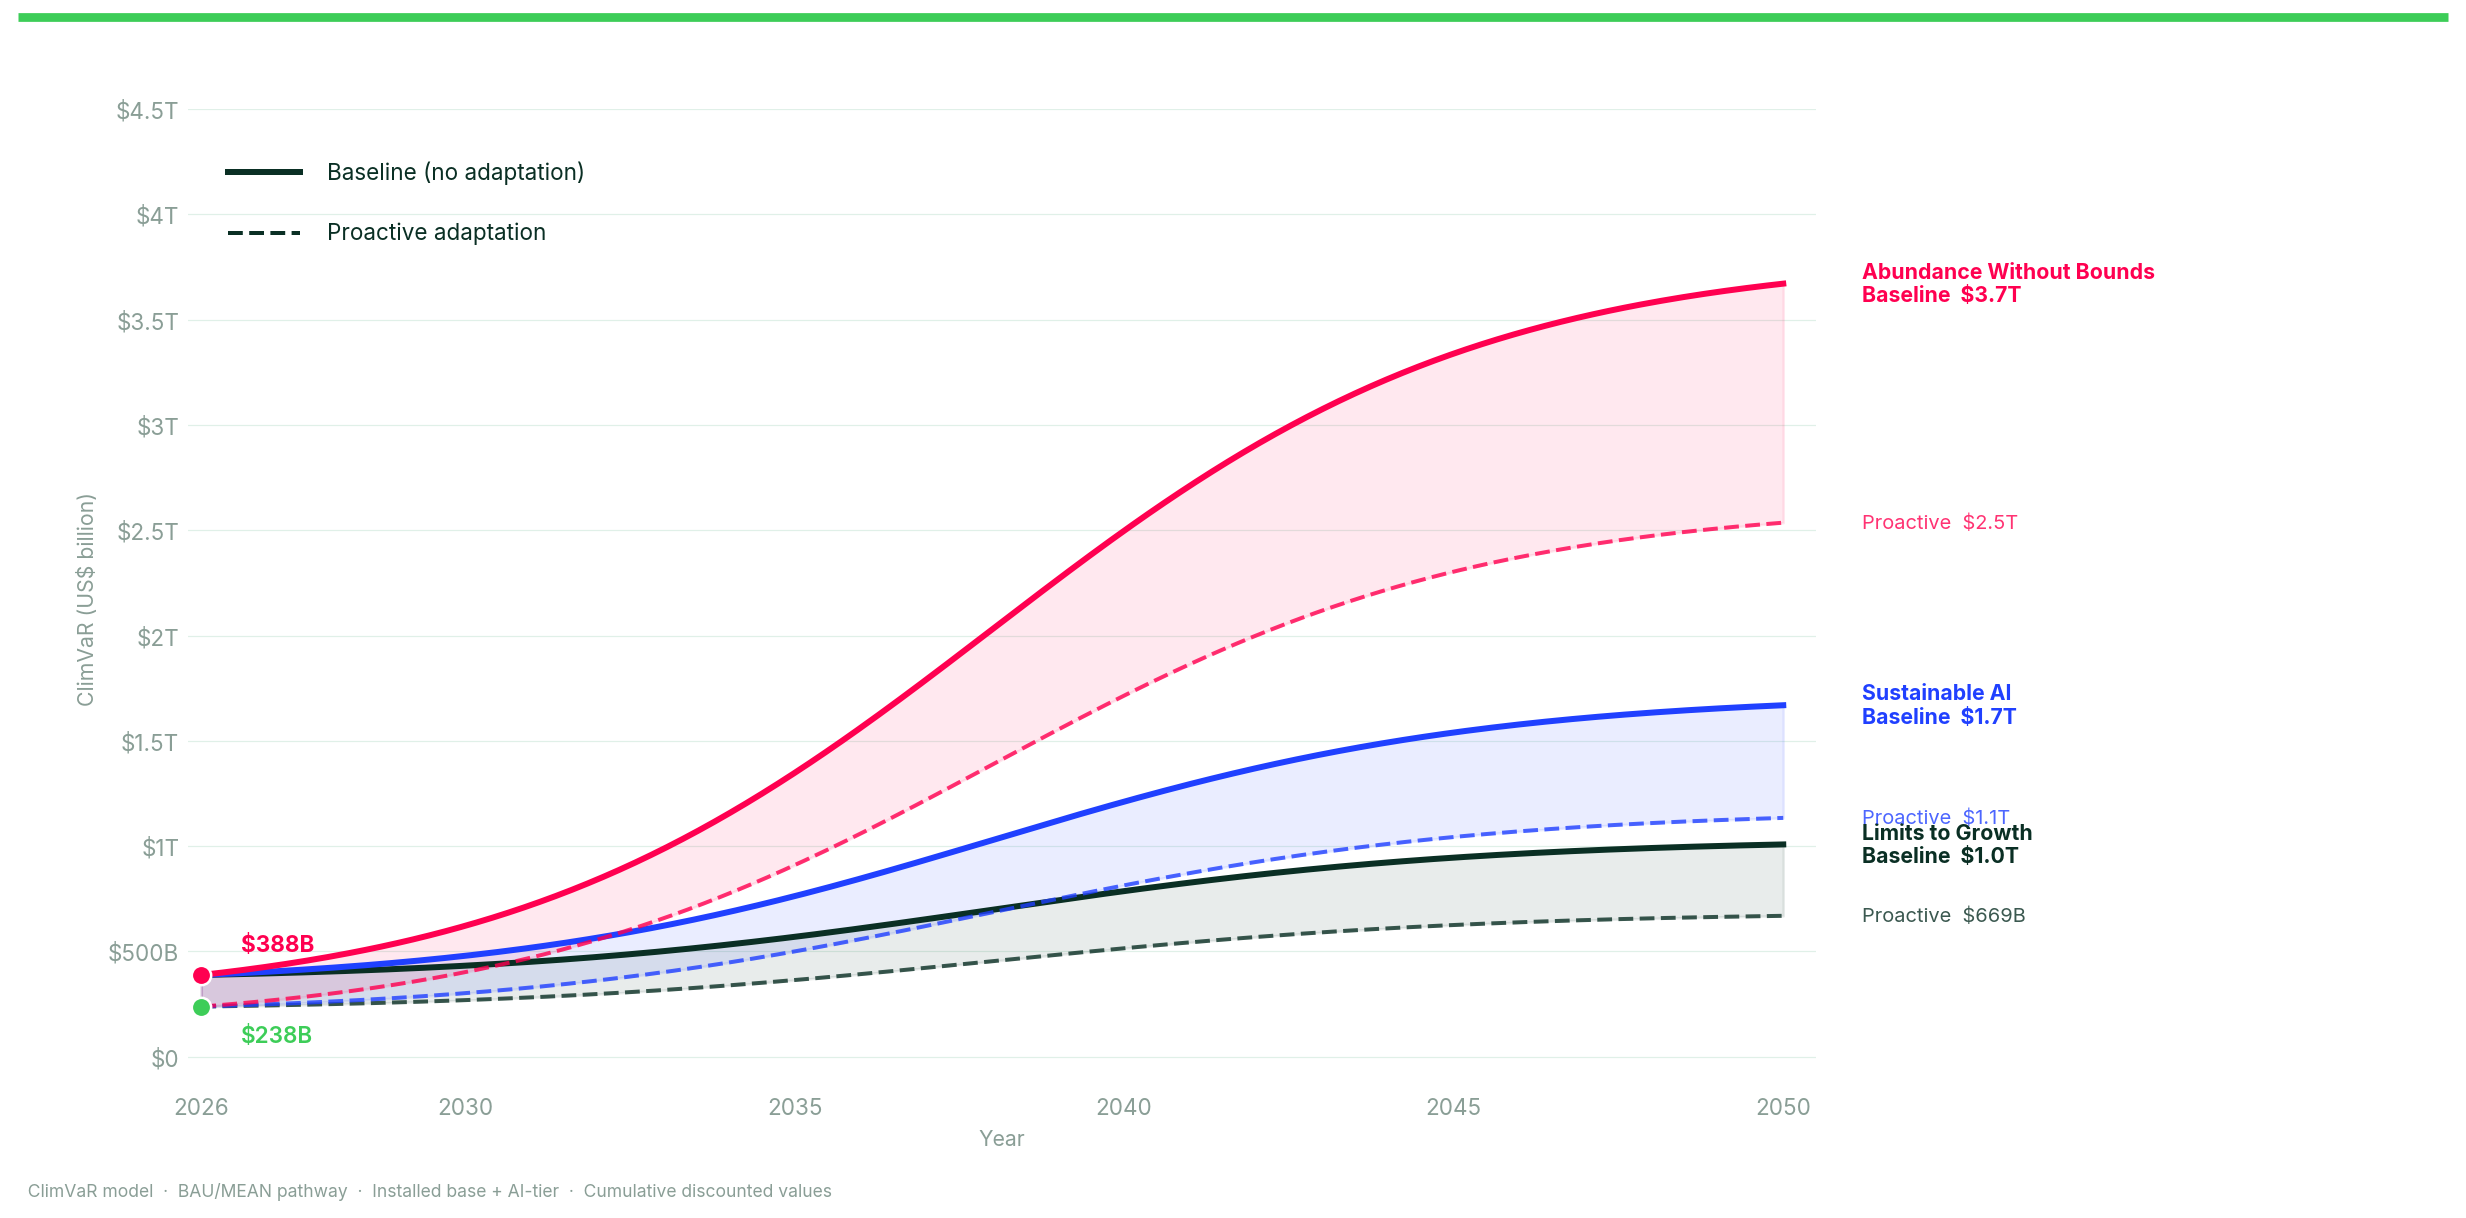
\includegraphics[width=\textwidth]{images/Image9.png}
\end{center}
\exhibitsource{Area ribbons: each colour band spans Baseline (solid) to Proactive (dashed) for one AI growth scenario. Ribbon width = adaptation value. End-values from ClimVaR V8 model, BAU pathway. Trajectories between endpoints are indicative.}

% ==============================================================================
% CASE STUDIES
% ==============================================================================
\clearpage\thispagestyle{chapterstart}

\subsection*{Three Facility Case Studies}
\sectionsubtitle{Translating aggregate patterns into site-level decisions}
\greensep

\begin{twocolbody}

\noindent Three prospective AI data centers produce ClimVaR intensities ranging from 37.6\% to 167\%, a 4.5$\times$ dispersion at site level. The Shapley decomposition and Leontief analysis produce their most concrete results at this scale. Abilene and Valence are identified facilities; Guangdong is a representative 100~MW allocation reflecting projected AI deployment in the Pearl River Delta---its results are indicative of the regional risk profile rather than a specific site assessment.

\end{twocolbody}

\vspace{2mm}
\exhibitcaption{23}{Three prospective AI facilities: site characteristics and ClimVaR decomposition (BAU/MEAN).}

\begin{center}
\datatablesetup
\begin{tabularx}{\textwidth}{>{\raggedright\arraybackslash}p{3.5cm} >{\centering\arraybackslash}X >{\centering\arraybackslash}X >{\centering\arraybackslash}X}
\toprule
\datatableheader
& \thd{Abilene, TX} & \thd{Valence, FR} & \thd{Guangdong, CN} \\
\midrule
Operator / Project & OpenAI Stargate & Sesterce sovereign & Pearl River Delta \\
Capacity & 2,800~MW & 100~MW & 100~MW \\
Enterprise value (V$_0$) & \$1.9B & \$2.1B & \$1.4B \\
PUE & 1.15 & 1.12 & 1.28 \\
\midrule
Business interruption & \$384M (43\%) & \$374M (11\%) & \$276M (53\%) \\
Cooling & \$336M (37\%) & \$459M (13\%) & \$96M (18\%) \\
Physical damage & \$143M (16\%) & \$2,678M (75\%) & \$29M (6\%) \\
Carbon & \$28M (3\%) & \$42M (1\%) & \$113M (22\%) \\
Heat productivity & \$11M (1\%) & \$6M ($<$1\%) & \$4M (1\%) \\
\midrule
\textbf{Total ClimVaR} & \textbf{\$902M} & \textbf{\$3,560M} & \textbf{\$517M} \\
\textbf{Intensity} & \textbf{46.5\%} & \textbf{167\%} & \textbf{37.6\%} \\
\bottomrule
\end{tabularx}
\datatableclear
\end{center}

\exhibitsource{V8 model results. BI includes direct + supply chain (Leontief). Enterprise values at facility level. Guangdong is a probabilistic allocation; results are indicative before site-specific due diligence.}

\begin{twocolbody}

\subsubsection*{Abilene, Texas --- The Supply Chain Problem}

The largest announced AI facility in the world carries a moderate 46.5\% ClimVaR intensity. But business interruption (43\%) and cooling (37\%) dominate, and the Shapley decomposition attributes 56\% of business interruption to tropical wind propagating through semiconductor and power equipment supply chains. Direct on-site risk accounts for less than 1\%. Abilene's risk is not where Abilene is---it is where its suppliers are.

\subsubsection*{Valence, France --- The Flood Trap}

A temperate European location perceived as ``safe'' carries 167\% ClimVaR intensity---its climate risk exceeds its entire enterprise value. River flood damage (\$2.7B, 75\% of total) dominates. The Rh\^{o}ne Valley's fluvial hazard profile, combined with the site's proximity to the river, produces an exposure that conventional risk screening does not flag. Valence demonstrates that climate risk assessment without granular hazard attribution produces false negatives. This result warrants site-specific due diligence before investment decisions; the model's archetype-based calibration may overstate or understate facility-specific flood exposure depending on exact elevation, flood defenses, and building specifications.

\subsubsection*{Guangdong, China --- The Triple Threat}

A more moderate 37.6\% intensity masks a three-channel interaction: business interruption (53\%), carbon (22\%), and cooling (18\%). The Pearl River Delta compounds typhoon exposure (supply chain), high grid carbon intensity (Scope~2), and subtropical heat stress. Guangdong is the prototypical case where no single adaptation lever reduces more than a quarter of total exposure. Effective risk reduction requires interventions across three channels simultaneously.

\end{twocolbody}

\vspace{2mm}
\exhibitcaption{24}{Hazard attribution (Shapley) and propagation pathway (Leontief) at three sites.}

\begin{center}
\datatablesetup
\begin{tabularx}{\textwidth}{>{\raggedright\arraybackslash}p{3.5cm} >{\centering\arraybackslash}X >{\centering\arraybackslash}X >{\centering\arraybackslash}X}
\toprule
\datatableheader
& \thd{Abilene, TX} & \thd{Valence, FR} & \thd{Guangdong, CN} \\
\midrule
\multicolumn{4}{l}{\textbf{BI: hazard attribution (Shapley)}} \\
Tropical wind / cyclone & 56\% & 52\% & 60\% \\
Storm (convective) & 24\% & 22\% & 27\% \\
Drought & 15\% & 23\% & 8\% \\
\midrule
\multicolumn{4}{l}{\textbf{BI: propagation pathway (Leontief)}} \\
Direct operations & $<$1\% & 2\% & 2\% \\
Supply chain (indirect) & $>$99\% & 98\% & 98\% \\
\midrule
\multicolumn{4}{l}{\textbf{Damage: dominant hazard}} \\
& Fire (97\%) & River flood (100\%) & Fire (79\%) \\
\bottomrule
\end{tabularx}
\datatableclear
\end{center}

\exhibitsource{Shapley: exact computation over 32 coalitions per facility. Leontief: OECD MRIOT 2023 vintage, ref.\ year 2020.}

\exhibitcaption{25}{Three sites, three risk profiles: channel decomposition at facility level.}
\begin{center}
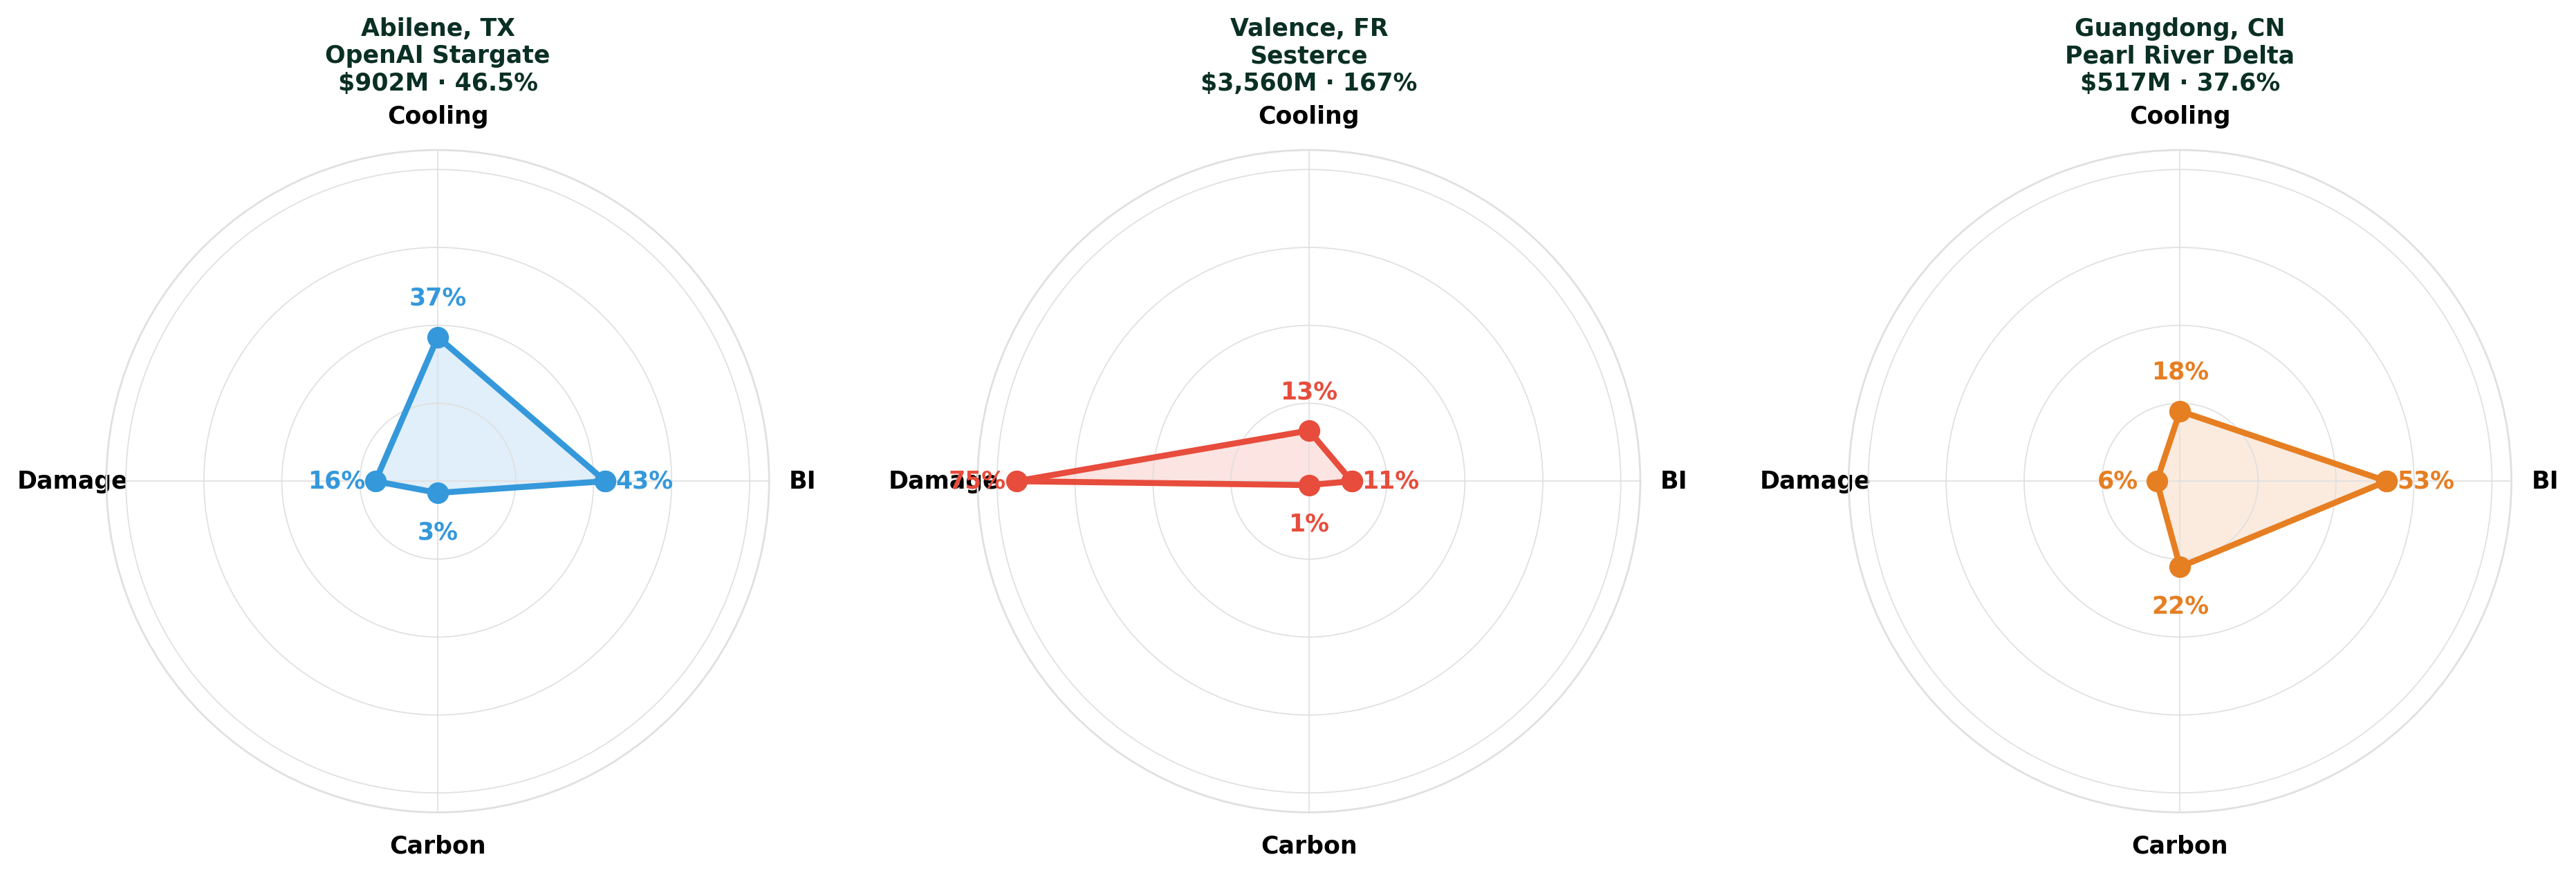
\includegraphics[width=\textwidth]{images/Image10.png}
\end{center}
\exhibitsource{Radar triptych: each polygon is one facility's channel fingerprint (\% of site-level ClimVaR). Abilene stretches toward BI and Cooling; Valence collapses onto Damage; Guangdong is the most balanced.}

\vspace{4mm}
\begin{tcolorbox}[colback=SEDarkGreen!5, colframe=SEGreen, title={\textcolor{SEGreen}{\textbf{From Analysis to Action: SE Advisory Services}}}, fonttitle=\sffamily\bfseries]
\small
The ClimVaR framework presented in this report is not a theoretical exercise---it is the analytical engine behind Schneider Electric's climate risk advisory offering. For operators and investors seeking to move from aggregate exposure figures to facility-level adaptation roadmaps, three service tiers are available:

\textbf{Portfolio Screening.} Rapid ClimVaR assessment across a portfolio of data centers, identifying the highest-risk facilities and the dominant risk channels at each site. Typical delivery: 4--6 weeks.

\textbf{Site-Level Deep Dive.} Full Shapley decomposition, Leontief supply chain mapping, and adaptation scenario modeling for individual facilities. Integrates site-specific engineering parameters (PUE, cooling architecture, grid connection) with the financial model. Typical delivery: 8--12 weeks per site.

\textbf{Strategic Adaptation Program.} Multi-year roadmap aligning capital allocation with risk reduction across a global portfolio. Includes MACC curve construction, greenfield vs.\ retrofit prioritization, and monitoring KPIs linked to ClimVaR reduction targets.

\vspace{1mm}
\noindent Contact: \texttt{advisory.services@se.com}
\end{tcolorbox}

% ==============================================================================
% DISCUSSION
% ==============================================================================
\clearpage\thispagestyle{chapterstart}

\subsection*{Discussion}
\sectionsubtitle{Interpretation, mechanisms, and implications}
\greensep

\begin{twocolbody}

\subsubsection*{The \$388 Billion Baseline in Context}

\noindent The US\$388~billion ClimVaR on the installed base (38.3\% of enterprise value) can be situated against three reference points. The WEF/S\&P aggregate of US\$3.3~trillion by 2055 operates at a different analytical level, but the order of magnitude is consistent when discounting and scope differences are accounted for \citep{wef2025}. XDI covers comparable facility counts but reports structural damage metrics rather than enterprise value loss; our framework extends this by adding cooling stress, carbon pricing, and supply chain propagation---channels that account for 65--75\% of total ClimVaR \citep{xdi2025}. Dietz et al.\ (2016) estimated 1.8\% of global financial assets at risk; the 38\% intensity for data centers reflects the sector's higher exposure through energy costs, uptime requirements, and supply chain concentration.

The \$388B figure represents a \textbf{lower bound} on total economic exposure. The framework quantifies private financial risk but does not capture systemic externalities: grid strain from concentrated AI load, water resource competition between data centers and agriculture, community displacement from extreme events, or the cascading economic effects of simultaneous service interruptions across interconnected facilities. These excluded channels would increase, not decrease, the total.

The gap between 38\% enterprise value erosion and zero in standard DCF valuations quantifies the mispricing. Concurrent work in portfolio management confirms this gap from the asset allocation side: \citet{luciani2026} show that physical climate risk lacks the standardized anchor metric equivalent to carbon intensity, and that reducing portfolio-level physical exposure beyond 10\% destabilizes diversified portfolios---the facility-level ClimVaR framework developed here is designed to provide precisely this missing metric.

\subsubsection*{The Supply Chain Multiplier}

The $\times$11 ratio of supply chain to direct business interruption is the most consequential finding for risk management practice. At all three case study sites, 98--99\% of business interruption propagates through supply chains rather than from direct on-site hazards. Taiwan accounts for over 60\% of advanced semiconductor fabrication; large power transformers carry 12--24 month lead times; high-bandwidth memory production concentrates in South Korea. A single typhoon disrupting TSMC operations would propagate through every data center in the global portfolio via the Leontief inverse \citep{verdantix2024}.

The Leontief framework assumes fixed technical coefficients---firms cannot reroute sourcing under stress. Long-duration disruptions are partially attenuated by adaptive behavior not captured in the model. The $\times$11 multiplier is an upper bound for prolonged disruptions and a reasonable estimate for acute shocks.

\subsubsection*{The Carbon Paradox}

Carbon is simultaneously the most responsive channel ($-$63\% via PPAs) and the most dependent on policy trajectories that operators do not control. Under BAU, a PPA investment generates a modest positive return by reducing Scope~2 costs. Under Net Zero Transition, the same PPA investment generates a return several times larger, because the carbon price against which it hedges rises sharply. The paradox is that PPA investment is rational even under BAU, because the BAU return is positive and the tail risk of NZT materializing is non-zero. Operators who delay PPA procurement are implicitly betting that ambitious climate policy will never arrive---a bet that the last five years of regulatory momentum makes increasingly difficult to justify.

\subsubsection*{The Decision Window}

The asymmetry between greenfield and retrofit adaptation costs is the most actionable finding for operators planning capital deployment. Integrating climate resilience at the design stage costs 15--20\% of CAPEX; retrofitting the same measures on commissioned facilities costs 40--60\%. This differential means that \textbf{every year of delayed adaptation permanently converts a greenfield opportunity into a future retrofit cost}. Under AWB, over \$4{,}600~billion in prospective AI infrastructure will be built within the next decade. The design choices being made now---location, cooling architecture, grid connection, supply chain sourcing---determine climate exposure for the next quarter century.

\subsubsection*{The Technology-Territory Equation}

The same investment---liquid cooling, PPA, microgrid---produces very different risk reductions depending on where it is deployed. Liquid cooling reduces ClimVaR by 40--50\% in hot climates (Gulf, Southeast Asia) but only 15--20\% in temperate locations where air cooling is already efficient. PPAs eliminate 60\%+ of the carbon channel in coal-dependent grids (China, parts of the US) but add little value in hydro-dominated systems (Nordics, Quebec). Supply chain diversification reduces business interruption by 20--30\% for facilities dependent on East Asian semiconductor supply, but is irrelevant for facilities with local sourcing. Standardizing adaptation playbooks across a global portfolio is an anti-pattern: the same dollar of investment generates 2--3$\times$ different returns depending on the regional channel fingerprint. The Shapley decomposition exists precisely to prevent this misallocation.

\subsubsection*{Physical Risk is Systemic}

The residual 61\% of ClimVaR that proactive adaptation cannot eliminate is not a failure of the framework---it reflects a structural reality. \citet{luciani2026} reach an analogous conclusion from the portfolio management side: ``physical risk is largely systemic, and systemic risks are difficult---if not impossible---to diversify.'' Their analysis shows that constraining physical risk exposure by even 10\% reduces investable portfolios to fewer than 200 stocks, with tracking error volatility rising by an order of magnitude compared to equivalent carbon constraints. Our facility-level results and their portfolio-level results converge on the same conclusion: the fraction of physical climate risk that individual actors can manage is bounded, and the remainder requires collective instruments---public risk-sharing, infrastructure stress tests, and regulatory frameworks calibrated to actual financial exposure.

\end{twocolbody}
